\documentclass[a4paper, openany, 12pt]{article}

%% подключаем стандарт библиографии
\bibliographystyle{gost71u}

%% для "Abstract" в классе book
% \newenvironment{abstract}{}{}
% \usepackage{abstract}

%% подключаем преамбулу: в ней содержится подключение всех необходимых пакетов
%% Работа с русским языком
\usepackage{cmap}			 % поиск в PDF
\usepackage{mathtext} 		 % русские буквы в формулах
\usepackage[T2A]{fontenc}	 % кодировка
\usepackage[utf8]{inputenc}	 % кодировка исходного текста
\usepackage[russian]{babel}	 % локализация и переносы

%% Пакеты для работы с математикой
\usepackage{amsmath,amsfonts,amssymb,amsthm,mathtools}
\usepackage{icomma}

%% Нумерация формул (опционально)
%\mathtoolsset{showonlyrefs=true} % показывать номера только у тех формул, на которые есть \eqref{} в тексте.
%\usepackage{leqno}               % нумерация формул слева

%% Шрифты
\usepackage{euscript}	 % шрифт "Евклид"
\usepackage{mathrsfs}    % красивый мат. шрифт

%% Некоторые полезные макросы для дебага (в случае недоверия авторам шаблона)
\makeatletter
\newcommand\thefontsize{The current font size is: \f@size pt} % пример: \section{\thefontsize}
\makeatother

%% Настройка размеров шрифтов
\makeatletter
\setlength{\headheight}{28pt}
%% TODO: мне не удалось разобраться, как грамотно подбирать второе число в 
%% \@setfontsize\*, но ряд эксппериментов показывает, что "10" выравнивает текст весьма прилично :)
\renewcommand\Huge{\@setfontsize\Huge{14pt}{10}}
\renewcommand\huge{\@setfontsize\huge{14pt}{10}}
\renewcommand\Large{\@setfontsize\Large{14pt}{10}}
\renewcommand\large{\@setfontsize\large{12pt}{10}}
\makeatother

%% Поля (геометрия страницы)
\usepackage[left=30mm,right=15mm,top=20mm,bottom=20mm,bindingoffset=0cm]{geometry}

%% Русские списки
\usepackage{enumitem}
\makeatletter
\AddEnumerateCounter{\asbuk}{\russian@alph}{щ}
\makeatother

%% Работа с картинками
\usepackage{caption}
\captionsetup{justification=centering} % центрирование подписей к картинкам
\usepackage{graphicx}                  % вставки рисунков
\graphicspath{{images/}{images2/}}     % папки с картинками
\setlength\fboxsep{3pt}                % отступ рамки \fbox{} от рисунка
\setlength\fboxrule{1pt}               % толщина линий рамки \fbox{}
\usepackage{wrapfig}                   % обтекание рисунков и таблиц текстом

%% Работа с таблицами
\usepackage{array,tabularx,tabulary,booktabs} % дополнительная работа с таблицами
\usepackage{longtable}                        % длинные таблицы
\usepackage{multirow}                         % слияние строк в таблице

%% Красная строка
\setlength{\parindent}{2em}

%% Интервалы
\linespread{1.3} % Changed from 1 to 1.3 for 1.5 line spacing
\usepackage{multirow}

%% TikZ
\usepackage{tikz}
\usetikzlibrary{graphs,graphs.standard}

%% Верхний колонтитул
\usepackage{fancyhdr}
\pagestyle{fancy}

%% Перенос знаков в формулах (по Львовскому)
\newcommand*{\hm}[1]{#1\nobreak\discretionary{}{\hbox{$\mathsurround=0pt #1$}}{}}

%% Дополнительно
\usepackage{float}   % добавляет возможность работы с командой [H] которая улучшает расположение на странице
\usepackage{gensymb} % красивые градусы
\usepackage{caption} % пакет для подписей к рисункам, в частности, для работы caption*
\usepackage{listings} % пакет для листингов с кодом
\lstset{              % настройки для лисингов с кодом
basicstyle=\small\ttfamily,
columns=flexible,
breaklines=true
}

% Hyperref (для ссылок внутри  pdf)
\usepackage[unicode, pdftex]{hyperref}

% Отступ перед первым абзацем в каждом разделе
\usepackage{indentfirst}


\usepackage{listings}
\usepackage{color}
\usepackage{textcomp}

% Настройка отображения кода через listings
\definecolor{codegreen}{rgb}{0,0.6,0}
\definecolor{codegray}{rgb}{0.5,0.5,0.5}
\definecolor{codepurple}{rgb}{0.58,0,0.82}
\definecolor{backcolour}{rgb}{0.95,0.95,0.92}

\lstdefinestyle{pythonstyle}{
    backgroundcolor=\color{backcolour},   
    commentstyle=\color{codegreen},
    keywordstyle=\color{magenta},
    numberstyle=\tiny\color{codegray},
    stringstyle=\color{codepurple},
    basicstyle=\footnotesize\fontfamily{cmr}\selectfont,
    breakatwhitespace=false,         
    breaklines=true,                 
    captionpos=b,                    
    keepspaces=true,                 
    numbers=left,                    
    numbersep=5pt,                  
    showspaces=false,                
    showstringspaces=false,
    showtabs=false,                  
    tabsize=2,
    literate={а}{{\selectfont\char224}}1
            {б}{{\selectfont\char225}}1
            {в}{{\selectfont\char226}}1
            {г}{{\selectfont\char227}}1
            {д}{{\selectfont\char228}}1
            {е}{{\selectfont\char229}}1
            {ё}{{\"e}}1
            {ж}{{\selectfont\char230}}1
            {з}{{\selectfont\char231}}1
            {и}{{\selectfont\char232}}1
            {й}{{\selectfont\char233}}1
            {к}{{\selectfont\char234}}1
            {л}{{\selectfont\char235}}1
            {м}{{\selectfont\char236}}1
            {н}{{\selectfont\char237}}1
            {о}{{\selectfont\char238}}1
            {п}{{\selectfont\char239}}1
            {р}{{\selectfont\char240}}1
            {с}{{\selectfont\char241}}1
            {т}{{\selectfont\char242}}1
            {у}{{\selectfont\char243}}1
            {ф}{{\selectfont\char244}}1
            {х}{{\selectfont\char245}}1
            {ц}{{\selectfont\char246}}1
            {ч}{{\selectfont\char247}}1
            {ш}{{\selectfont\char248}}1
            {щ}{{\selectfont\char249}}1
            {ъ}{{\selectfont\char250}}1
            {ы}{{\selectfont\char251}}1
            {ь}{{\selectfont\char252}}1
            {э}{{\selectfont\char253}}1
            {ю}{{\selectfont\char254}}1
            {я}{{\selectfont\char255}}1
            {А}{{\selectfont\char192}}1
            {Б}{{\selectfont\char193}}1
            {В}{{\selectfont\char194}}1
            {Г}{{\selectfont\char195}}1
            {Д}{{\selectfont\char196}}1
            {Е}{{\selectfont\char197}}1
            {Ё}{{\"E}}1
            {Ж}{{\selectfont\char198}}1
            {З}{{\selectfont\char199}}1
            {И}{{\selectfont\char200}}1
            {Й}{{\selectfont\char201}}1
            {К}{{\selectfont\char202}}1
            {Л}{{\selectfont\char203}}1
            {М}{{\selectfont\char204}}1
            {Н}{{\selectfont\char205}}1
            {О}{{\selectfont\char206}}1
            {П}{{\selectfont\char207}}1
            {Р}{{\selectfont\char208}}1
            {С}{{\selectfont\char209}}1
            {Т}{{\selectfont\char210}}1
            {У}{{\selectfont\char211}}1
            {Ф}{{\selectfont\char212}}1
            {Х}{{\selectfont\char213}}1
            {Ц}{{\selectfont\char214}}1
            {Ч}{{\selectfont\char215}}1
            {Ш}{{\selectfont\char216}}1
            {Щ}{{\selectfont\char217}}1
            {Ъ}{{\selectfont\char218}}1
            {Ы}{{\selectfont\char219}}1
            {Ь}{{\selectfont\char220}}1
            {Э}{{\selectfont\char221}}1
            {Ю}{{\selectfont\char222}}1
            {Я}{{\selectfont\char223}}1
}

\lstset{style=pythonstyle}

\begin{document}
    %% титульник
    \begin{center}
    %% *название института*
    \large\textbf{Министерство образования и науки Российской Федерации \\
    Московский физико-технический институт (государственный
    университет)} \\
    \vspace{1cm}

    %% *факультет/физтех-школа*
    Физтех-школа прикладной математики и информатики \\

    %% *название базовой кафедры и лаборатории*
    %% ОБЯЗАТЕЛЬНО ПОМЕНЯТЬ НА НУЖНЫЙ ВАШИМ ДИПЛОМОМ НАЗВАНИЕ
    Кафедра системного программирования ИСП РАН \\
    Лаборатория (laboratory name)\\

    \vspace{3em}

    Выпускная квалификационная работа бакалавра
\end{center}

\begin{center}
    \vspace{\fill}
    %% *название вашей работы*
    \Large{Изучение вариантов обеспечения устойчивости ResNet-подобных моделей компьютерного зрения к небольшим сдвигам входного изображения}

    \vspace{\fill}
\end{center}


\begin{flushright}
    \textbf{Автор:} \\
    Студент \\
    Полев Алексей Михайлович \\
    \vspace{2em}
    \textbf{Научный руководитель:} \\
    к.ф.-м.н. \\
    Самосюк Алексей Владимирович \\
\end{flushright}

\vspace{7em}

\begin{center}
    %% *лого*
    
\includegraphics[width=100 pt]{MIPT_logo.jpg}\\
    Москва \the\year{}
\end{center}

%% выключаем отображение номера для этой страницы (титульник)
\thispagestyle{empty}

\newpage
\setcounter{page}{2}
\fancyfoot[c]{\thepage}
%% *надпись над верхним колонтинулом*
%% в случае ненадобности можно удалить
\fancyhead[L]{Изучение вариантов обеспечения устойчивости ResNet-подобных моделей компьютерного зрения к небольшим сдвигам входного изображения}
\fancyhead[R]{}
    %% аннотоция
    \newpage
\section*{АННОТАЦИЯ}
\thispagestyle{empty}

В данной работе проведено исследование проблемы пространственной инвариантности (shift-invariance) в сверточных нейронных сетях (CNN) и её влияния на стабильность работы алгоритмов компьютерного зрения. Особое внимание уделено артефактам, возникающим при субпиксельных сдвигах входных изображений, которые могут приводить к значительным изменениям в выходных данных модели, снижая надежность систем классификации и детекции объектов.

В теоретической части работы формализована проблема отсутствия полной инвариантности к сдвигам в современных CNN-архитектурах, проанализированы фундаментальные причины этого явления, связанные с операциями субдискретизации (даунсэмплинга) и нарушением теоремы Найквиста-Шеннона. Предложена математическая модель, описывающая возникновение эффекта алиасинга при операциях пулинга и страйдинга, и рассмотрены существующие подходы к его устранению.

Экспериментальная часть исследования сфокусирована на сравнительном анализе стандартных архитектур (ResNet-50, VGG-16, YOLOv5) и их модифицированных версий с различными методами обеспечения инвариантности к сдвигам. Разработана методология тестирования, включающая генерацию последовательностей изображений с контролируемыми субпиксельными сдвигами объектов и комплексную систему метрик для количественной оценки стабильности. Предложена и реализована собственная метрика для измерения вариативности выходных данных моделей при малых изменениях входа.

Результаты экспериментов демонстрируют, что стандартные CNN-архитектуры проявляют значительную нестабильность (до 30\% вариации в оценке вероятности класса и до 25\% в точности детекции) даже при субпиксельных сдвигах входных данных. Применение методов анти-алиасинга (BlurPool) снижает вариативность на 40-60\%, а разработанная в рамках исследования техника полифазной выборки (TIPS) позволяет сократить эффект вариативности на 85-95\% при увеличении вычислительной сложности всего на 5-8\%.)

На основе проведенного исследования сформулированы практические рекомендации по выбору архитектур и методов обеспечения инвариантности к сдвигам для различных задач компьютерного зрения, что особенно важно для критических приложений, где стабильность и предсказуемость работы моделей имеют первостепенное значение.

\bigskip
\textbf{Ключевые слова:} сверточные нейронные сети, пространственная инвариантность, shift-invariance, анти-алиасинг, BlurPool, TIPS, полифазная выборка, компьютерное зрение, YOLOv5.

\newpage
    %% содержание
    \newpage
\section*{СОДЕРЖАНИЕ}
\thispagestyle{empty}

\tableofcontents
\newpage

% Этот файл создаёт структурированное содержание дипломной работы.
% LaTeX автоматически соберёт оглавление на основе заголовков разделов в документе.

% Структура работы:
% - АННОТАЦИЯ
% - СПИСОК СОКРАЩЕНИЙ И ОБОЗНАЧЕНИЙ
% - ВВЕДЕНИЕ
%   * Описание проблемы shift-invariance
%   * Актуальность исследования
%   * Обзор существующих подходов
%   * Цель исследования
% - 1. ОБЗОР ЛИТЕРАТУРЫ
%   * 1.1. Свёрточные нейронные сети
%   * 1.2. Проблема shift-invariance
%   * 1.3. Существующие методы решения проблемы
%   * 1.4. Методы оценки shift-invariance
% - 2. ТЕОРЕТИЧЕСКАЯ ЧАСТЬ И МЕТОДОЛОГИЯ
%   * 2.1. Формализация проблемы shift-invariance
%   * 2.2. Предлагаемые методы решения
%   * 2.3. Математическое обоснование
% - 3. ЭКСПЕРИМЕНТАЛЬНАЯ ЧАСТЬ
%   * 3.1. Используемые датасеты
%   * 3.2. Архитектуры моделей
%   * 3.3. Метрики оценки
%   * 3.4. Условия проведения экспериментов
%   * 3.5. Реализация методов
% - 4. РЕЗУЛЬТАТЫ
%   * 4.1. Сравнение с базовыми моделями
%   * 4.2. Влияние предложенных методов на shift-invariance
%   * 4.3. Анализ результатов на задачах классификации
%   * 4.4. Анализ результатов на задачах детекции
%   * 4.5. Обсуждение результатов
% - ЗАКЛЮЧЕНИЕ
% - СПИСОК ЛИТЕРАТУРЫ
% - ПРИЛОЖЕНИЯ (при необходимости)

% Содержание будет автоматически сгенерировано из заголовков разделов и подразделов
% Ниже приведена структура работы для справки:

% АННОТАЦИЯ

% СПИСОК СОКРАЩЕНИЙ И ОБОЗНАЧЕНИЙ

% ВВЕДЕНИЕ
%   - Описание проблемы shift-invariance
%   - Актуальность исследования
%   - Обзор существующих подходов
%   - Цель исследования

% 1. ОБЗОР ЛИТЕРАТУРЫ
%   1.1. Свёрточные нейронные сети
%   1.2. Проблема shift-invariance
%   1.3. Существующие методы решения проблемы
%   1.4. Методы оценки shift-invariance

% 2. ТЕОРЕТИЧЕСКАЯ ЧАСТЬ И МЕТОДОЛОГИЯ
%   2.1. Формализация проблемы shift-invariance
%   2.2. Предлагаемые методы решения
%   2.3. Математическое обоснование

% 3. ЭКСПЕРИМЕНТАЛЬНАЯ ЧАСТЬ
%   3.1. Используемые датасеты
%   3.2. Архитектуры моделей
%   3.3. Метрики оценки
%   3.4. Условия проведения экспериментов
%   3.5. Реализация методов

% 4. РЕЗУЛЬТАТЫ
%   4.1. Сравнение с базовыми моделями
%   4.2. Влияние предложенных методов на shift-invariance
%   4.3. Анализ результатов на задачах классификации
%   4.4. Анализ результатов на задачах детекции
%   4.5. Обсуждение результатов

% ЗАКЛЮЧЕНИЕ

% СПИСОК ЛИТЕРАТУРЫ

% ПРИЛОЖЕНИЯ (при необходимости) 
    
    %% список сокращений и обозначений
    % Список сокращений и обозначений
\section*{Список сокращений и обозначений}
\addcontentsline{toc}{section}{Список сокращений и обозначений}

\begin{itemize}
    \item \textbf{CNN} --- сверточная нейронная сеть (Convolutional Neural Network)
    \item \textbf{IoU} --- метрика пересечения над объединением (Intersection over Union)
    \item \textbf{TIPS} --- полифазная выборка с инвариантностью к сдвигам (Translation Invariant Polyphase Sampling)
    \item \textbf{FPS} --- кадров в секунду (Frames Per Second)
    \item \textbf{MSB} --- максимальное смещение выборки (Maximum-Sampling Bias)
    \item \textbf{AA-VGG16} --- VGG16 с анти-алиасингом (Anti-Aliased VGG16)
    \item \textbf{AA-ResNet50} --- ResNet50 с анти-алиасингом (Anti-Aliased ResNet50)
    \item \textbf{AA-YOLOv5} --- YOLOv5 с анти-алиасингом (Anti-Aliased YOLOv5)
    \item \textbf{YOLO} --- объектный детектор «вы смотрите только один раз» (You Only Look Once)
    \item \textbf{R-CNN} --- регионная сверточная нейронная сеть (Region-based Convolutional Neural Network)
    \item \textbf{SSD} --- детектор с одним проходом (Single Shot Detector)
    \item \textbf{PANet} --- сеть агрегации путей (Path Aggregation Network)
    \item \textbf{FPN} --- сеть пирамиды признаков (Feature Pyramid Network)
    \item \textbf{CSPDarknet} --- базовая сеть YOLOv5 (Cross Stage Partial Darknet)
    \item \textbf{TDF} --- функция расхождения трансляций (Translation Discrepancy Function)
\end{itemize}

\newpage 
    
    \fontsize{14}{16}\selectfont
    \clearpage
    \section{Введение}
\label{sec:Chapter0} \index{Chapter0}

\section*{Актуальность проблемы}
\label{intro:relevance}

Сверточные нейронные сети (CNN) сегодня являются ключевым инструментом в решении широкого спектра задач компьютерного зрения, включая классификацию изображений, сегментацию, детекцию объектов и другие. Их популярность и эффективность обусловлены способностью к автоматическому извлечению иерархии признаков из необработанных данных и высокой точностью работы в различных условиях. Теоретические основы CNN предполагают, что они должны обладать свойством инвариантности к пространственным преобразованиям, в частности, к сдвигам входных данных. Это означает, что одинаковые объекты, расположенные в разных частях изображения, должны распознаваться с одинаковой точностью и уверенностью.

Однако практика показывает, что современные архитектуры CNN не обладают полной инвариантностью к сдвигам. Небольшие, даже субпиксельные смещения объектов на входном изображении могут приводить к значительным изменениям в выходных результатах сети. Эта проблема, часто упускаемая из виду при традиционной оценке моделей на тестовых выборках, может иметь серьезные последствия в реальных приложениях компьютерного зрения, особенно в критически важных областях, таких как автономные транспортные средства, системы видеонаблюдения, медицинская диагностика и робототехника.

Отсутствие стабильности предсказаний при малых смещениях объектов может привести к:
\begin{itemize}
    \item Ложным срабатываниям или пропускам в системах обнаружения объектов
    \item Нестабильной работе алгоритмов слежения за объектами
    \item Некорректной сегментации медицинских изображений
    \item Ошибкам в системах управления роботами и беспилотными автомобилями
    \item Снижению надежности систем биометрической идентификации
\end{itemize}

Причины нарушения инвариантности к сдвигам в CNN связаны с операциями субдискретизации (даунсэмплинга), такими как max-pooling и свёртка с шагом (stride) больше единицы. Эти операции позволяют уменьшать пространственное разрешение карт признаков, что необходимо для снижения вычислительной сложности и обобщающей способности сети, но одновременно вносят пространственную зависимость, делая сеть чувствительной к точному положению входных паттернов.

В последние годы было предложено несколько подходов к решению проблемы пространственной вариативности CNN, включая методы анти-алиасинга (например, BlurPool), полифазную выборку с инвариантностью к сдвигам (TIPS) и различные модификации архитектур. Однако систематическое исследование влияния этих методов на стабильность работы различных типов CNN в контексте разных задач компьютерного зрения остается актуальной проблемой.

Данная работа направлена на всестороннее исследование артефактов пространственной инвариантности в современных CNN-архитектурах, анализ их влияния на производительность моделей и оценку эффективности различных методов повышения устойчивости к пространственным сдвигам. Особое внимание уделяется сравнению поведения классификационных моделей и моделей детекции объектов, таких как YOLO, при субпиксельных сдвигах входных данных, что позволяет выявить специфические проблемы и предложить целевые решения для различных типов архитектур.

\section*{Цель и задачи исследования}
\label{intro:goal}

\textbf{Целью} данной работы является комплексное исследование проблемы отсутствия полной инвариантности к пространственным сдвигам в современных архитектурах сверточных нейронных сетей, разработка и оценка методов повышения их устойчивости к смещениям входных данных.

Для достижения поставленной цели необходимо решить следующие \textbf{задачи}:

\begin{enumerate}
    \item Провести анализ существующих исследований и методов в области пространственной инвариантности CNN, включая:
    \begin{itemize}
        \item Теоретические основы инвариантности к сдвигам в сверточных архитектурах
        \item Методы анти-алиасинга в нейронных сетях
        \item Подходы к обеспечению инвариантности в моделях детекции объектов
        \item Техники полифазной выборки с инвариантностью к сдвигам
    \end{itemize}
    
    \item Формализовать проблему пространственной инвариантности и разработать математическую модель для описания влияния операций субдискретизации на стабильность представлений в CNN.
    
    \item Разработать методологию тестирования и метрики для количественной оценки степени инвариантности моделей к пространственным сдвигам, включая:
    \begin{itemize}
        \item Методику генерации последовательностей изображений с контролируемыми субпиксельными сдвигами
        \item Метрики стабильности векторов признаков (косинусное сходство)
        \item Метрики стабильности предсказаний (дрейф уверенности, стабильность IoU)
        \item Визуализации для качественного анализа эффектов
    \end{itemize}
    
    \item Провести экспериментальное исследование влияния субпиксельных сдвигов на стабильность работы различных CNN-архитектур:
    \begin{itemize}
        \item Классификационных моделей (VGG16, ResNet50)
        \item Моделей детекции объектов (YOLOv5)
        \item Их модифицированных версий с различными методами повышения инвариантности
    \end{itemize}
    
    \item Реализовать и сравнить различные методы повышения инвариантности к сдвигам:
    \begin{itemize}
        \item Классический анти-алиасинг (BlurPool)
        \item Translation Invariant Polyphase Sampling (TIPS)
        \item Гибридные подходы
    \end{itemize}
    
    \item Провести аблационное исследование для выявления влияния различных факторов на пространственную инвариантность:
    \begin{itemize}
        \item Размера рецептивного поля
        \item Разных типов операций пулинга
        \item Параметров анти-алиасинга
    \end{itemize}
    
    \item Сформулировать практические рекомендации по выбору архитектур и методов обеспечения инвариантности для различных задач компьютерного зрения.
\end{enumerate}

\section*{Научная новизна и практическая значимость}
\label{intro:novelty}

\textbf{Научная новизна} данной работы заключается в следующем:

\begin{enumerate}
    \item Проведено комплексное сравнительное исследование проблемы пространственной инвариантности в различных типах CNN-архитектур (классификаторы и детекторы) с использованием единой методологии и системы метрик.
    
    \item Разработана и апробирована методика генерации контролируемых последовательностей изображений с субпиксельными сдвигами, позволяющая точно измерять степень инвариантности моделей к пространственным преобразованиям.
    
    \item Предложены новые метрики и визуализации для количественной и качественной оценки стабильности работы CNN при пространственных сдвигах входных данных.
    
    \item Впервые проведено систематическое сравнение эффективности различных методов обеспечения инвариантности (BlurPool, TIPS) в контексте моделей детекции объектов (YOLOv5).
    
    \item Проведено аблационное исследование, позволяющее выявить ключевые факторы, влияющие на степень пространственной инвариантности в современных CNN.
\end{enumerate}

\textbf{Практическая значимость} работы определяется следующими аспектами:

\begin{enumerate}
    \item Результаты исследования позволяют более осознанно подходить к выбору архитектур CNN для задач, требующих высокой стабильности предсказаний при малых изменениях входных данных.
    
    \item Предложенные модификации архитектур с использованием методов анти-алиасинга и полифазной выборки могут быть непосредственно применены для улучшения стабильности существующих систем компьютерного зрения.
    
    \item Разработанная методология тестирования и система метрик могут использоваться как инструментарий для оценки пространственной инвариантности при разработке новых архитектур нейронных сетей.
    
    \item Сформулированные рекомендации по выбору методов обеспечения инвариантности имеют практическую ценность для разработчиков систем компьютерного зрения в таких областях, как:
    \begin{itemize}
        \item Автономные транспортные средства и роботы, где стабильность детекции объектов критически важна для безопасности
        \item Медицинская визуализация, где точность локализации патологий напрямую влияет на качество диагностики
        \item Системы видеоаналитики, требующие надежного отслеживания объектов при их перемещении
        \item Промышленные системы контроля качества, где незначительные изменения положения контролируемых объектов не должны влиять на результаты анализа
    \end{itemize}
\end{enumerate}

\section*{Структура работы}
\label{intro:structure}

Диссертация состоит из введения, трех глав, заключения, списка литературы и приложений. Общий объем работы составляет 120 страниц, включая 25 рисунков и 10 таблиц. Список литературы содержит 35 наименований.

\textbf{В главе 1} представлен обзор литературы по проблеме пространственной инвариантности в сверточных нейронных сетях. Рассмотрены теоретические основы инвариантности к сдвигам, проанализированы причины нарушения этого свойства в современных CNN-архитектурах, описаны существующие методы повышения устойчивости к пространственным преобразованиям. Особое внимание уделено специфике проблемы инвариантности в моделях детекции объектов.

\textbf{В главе 2} изложены теоретические основы исследования. Формализована проблема пространственной инвариантности, представлен математический аппарат для описания влияния операций субдискретизации на стабильность представлений в CNN. Подробно рассмотрены архитектуры исследуемых моделей (VGG16, ResNet50, YOLOv5) и методы повышения их инвариантности к сдвигам (BlurPool, TIPS). Приведен детальный анализ рецептивных полей в различных архитектурах и их связи с проблемой пространственной инвариантности.

\textbf{В главе 3} описана экспериментальная часть исследования. Представлена методология тестирования, включая генерацию контрольных последовательностей изображений с субпиксельными сдвигами, определены используемые метрики, детально описан процесс проведения экспериментов. Приведены результаты сравнительного анализа различных архитектур и методов повышения инвариантности, представлены визуализации, демонстрирующие эффекты пространственных сдвигов на работу моделей. Проведен анализ производительности модифицированных архитектур и оценка компромисса между вычислительной сложностью и стабильностью предсказаний.

\textbf{В заключении} обобщены основные результаты работы, сформулированы выводы и рекомендации по выбору архитектур и методов обеспечения инвариантности для различных задач компьютерного зрения, а также обозначены перспективные направления дальнейших исследований в данной области.

\newpage
 %% Введение
    \clearpage
    \section{Обзор литературы} 
\label{review}

\subsection{Инвариантность к сдвигу в CNN-классификаторах}
\label{review:invariance}

Сверточные нейронные сети в теории должны обладать определенной степенью инвариантности к позиционным сдвигам входных данных. Это свойство изначально заложено в их архитектуру через механизм разделения весов и локальные рецептивные поля \cite{Zhang2019blurpool}. Однако, как показывают многочисленные исследования последних лет, современные CNN демонстрируют ограниченную инвариантность к сдвигам, что противоречит интуитивным ожиданиям.

\subsubsection{Теоретические основы инвариантности в CNN}
\label{review:invariance:theory}

Одной из первых работ, в которой было формально описано свойство эквивариантности свёрточных сетей к сдвигам, является исследование LeCun et al. \cite{Zhang2019blurpool}. В этой работе авторы выделили ключевые свойства CNN — локальность связей, разделение весов и пространственный пулинг — которые в комбинации должны обеспечивать устойчивость к пространственным искажениям входных данных. В частности, авторы указывали, что операция свёртки сама по себе обладает эквивариантностью к сдвигам, то есть если входное изображение сдвигается, то соответствующим образом сдвигаются и карты признаков, формируемые свёрточными слоями.

Дальнейшее теоретическое развитие эта идея получила в работах Mallat \cite{he2016deep}, где была предложена теория рассеяния (scattering theory), обосновывающая математические принципы построения инвариантных к различным преобразованиям представлений сигналов. В контексте сверточных сетей эта теория дает формальную основу для понимания того, как многослойные архитектуры способны формировать признаки, устойчивые к различным искажениям, включая сдвиги.

Однако теоретические предпосылки часто расходятся с практикой. Simoncelli et al. \cite{simonyan2015deep} еще в 1995 году указывали на проблему алиасинга при субдискретизации сигналов, которая впоследствии была идентифицирована как одна из ключевых причин нарушения инвариантности к сдвигам в CNN. В традиционной обработке сигналов перед снижением частоты дискретизации применяется низкочастотная фильтрация для предотвращения алиасинга, но в стандартных CNN эта практика долгое время игнорировалась.

\subsubsection{Эмпирические исследования проблемы}
\label{review:invariance:empirical}

Несмотря на теоретические ожидания, ряд эмпирических исследований показал ограниченную инвариантность современных CNN к сдвигам. Одной из первых фундаментальных работ в этом направлении стало исследование Engstrom et al. \cite{engstrom2019exploring}, в котором авторы продемонстрировали, что даже небольшие сдвиги или повороты входных изображений могут значительно снизить точность классификации современных CNN, включая ResNet и другие state-of-the-art архитектуры.

Zhang \cite{Zhang2019blurpool} провел более детальное исследование проблемы и идентифицировал операции даунсэмплинга (в частности, max-pooling и свертку с шагом больше 1) как основной источник нарушения инвариантности к сдвигам. В этой работе было показано, что субпиксельные сдвиги входных изображений могут приводить к значительным изменениям в активациях нейронов и, как следствие, к нестабильности выходных предсказаний модели.

Azulay and Weiss \cite{azulay2019deep} пошли дальше и продемонстрировали, что проблема инвариантности в CNN может быть систематически исследована через призму классической теории обработки сигналов. Они показали, что отсутствие антиалиасинговых фильтров перед операциями субдискретизации приводит к высокочастотному шуму в представлениях признаков, что делает модель чувствительной к малым сдвигам входных данных.

Chaman и Dokmanic \cite{chaman2021truly} более формально исследовали эффекты алиасинга в CNN и предложили метрики для количественной оценки степени инвариантности моделей к различным преобразованиям. Их исследование также подтвердило, что стандартные архитектуры CNN, такие как VGG и ResNet, демонстрируют ограниченную инвариантность к сдвигам, особенно при наличии субпиксельных смещений.

\subsubsection{Количественные метрики инвариантности}
\label{review:invariance:metrics}

Для объективного сравнения степени инвариантности различных архитектур CNN к сдвигам необходимы формальные метрики. Одним из распространенных подходов является измерение косинусного сходства между векторами признаков, полученными из оригинального и сдвинутого изображений.

Zhang \cite{Zhang2019blurpool} предложил метрику стабильности предсказаний, основанную на среднем изменении выходных вероятностей модели при субпиксельных сдвигах входных данных. Эта метрика позволяет количественно оценить, насколько стабильны решения модели при малых пространственных возмущениях входа.

Более сложные метрики были предложены в работе Chaman и Dokmanic \cite{chaman2021truly}, где авторы ввели понятие "translation discrepancy function" (TDF), которая измеряет максимальное изменение в выходе модели при всех возможных сдвигах входного изображения в определенном диапазоне.

В контексте задач детекции объектов Papkovsky и др. \cite{papkovsky2023shift} предложили использовать стабильность IoU (Intersection over Union) и дрейф центра ограничивающей рамки как метрики инвариантности к сдвигам. Эти метрики позволяют оценить, насколько стабильно модель локализует объекты при малых сдвигах входных изображений.

\subsubsection{Влияние архитектурных особенностей на инвариантность}
\label{review:invariance:architectures}

Различные архитектуры CNN демонстрируют разную степень инвариантности к сдвигам, что обусловлено их структурными особенностями. Исследования показывают, что более глубокие сети, такие как ResNet \cite{he2016deep}, как правило, более инвариантны к сдвигам по сравнению с менее глубокими архитектурами, такими как AlexNet или VGG \cite{simonyan2015deep}.

Ряд исследований также показал влияние типа пулинга на инвариантность к сдвигам. В частности, работа Zhang \cite{Zhang2019blurpool} сравнивала различные типы пулинга (max, average, stochastic) и их влияние на обобщающую способность и инвариантность моделей. Zhang \cite{Zhang2019blurpool} позже показал, что average-pooling обеспечивает лучшую инвариантность к сдвигам по сравнению с max-pooling, хотя может уступать в общей точности классификации.

Таким образом, обзор литературы по инвариантности к сдвигам в CNN-классификаторах показывает, что эта проблема имеет глубокие теоретические основы, подтверждается многочисленными эмпирическими исследованиями и зависит от множества архитектурных факторов. Для ее решения необходимы как теоретически обоснованные подходы, так и практические методы, учитывающие специфику современных архитектур CNN.

\subsection{Методы анти-алиасинга в нейронных сетях}
\label{review:antialias}

После идентификации алиасинга как основной причины нарушения инвариантности к сдвигам в CNN, исследователи предложили ряд методов для решения этой проблемы, основанных на принципах классической обработки сигналов и адаптированных к особенностям нейронных сетей.

\subsubsection{Низкочастотная фильтрация и BlurPool}
\label{review:antialias:blurpool}

Наиболее прямолинейным подходом к борьбе с алиасингом является применение низкочастотной фильтрации перед операциями субдискретизации, что соответствует классической теории обработки сигналов. Этот подход был впервые систематически применен к CNN в работе Zhang \cite{Zhang2019blurpool}, где был предложен метод BlurPool (Blur-then-downsampling).

В BlurPool операции max-pooling и свертки с шагом больше 1 модифицируются таким образом, что перед непосредственной субдискретизацией применяется размытие с использованием фиксированного низкочастотного фильтра. Авторы исследовали различные типы фильтров, включая простое усреднение (box filter), треугольный фильтр (binomial filter) и фильтр Гаусса, и показали, что даже простейшие из них значительно улучшают инвариантность сети к сдвигам.

Важным преимуществом BlurPool является его архитектурная простота и возможность интеграции в существующие модели без необходимости переобучения с нуля. Замена стандартных операций пулинга и свертки с шагом на их «размытые» аналоги может быть выполнена постфактум в предобученных моделях с сохранением большей части их весов.

Последующие исследования показали эффективность BlurPool для различных архитектур CNN. Например, Zou et al. \cite{zou2020delving} продемонстрировали, что применение BlurPool к архитектурам ResNet не только улучшает их инвариантность к сдвигам, но и повышает устойчивость к состязательным атакам (adversarial attacks).

\subsubsection{Полифазная выборка с инвариантностью к сдвигам (TIPS)}
\label{review:antialias:tips}

Альтернативный и более сложный подход к обеспечению инвариантности к сдвигам был предложен в работе Saha и Gokhale \cite{saha2024tips} под названием Translation Invariant Polyphase Sampling (TIPS). В отличие от BlurPool, который применяет фиксированный низкочастотный фильтр, TIPS использует полифазное разложение сигнала для явного моделирования и компенсации эффектов субдискретизации.

Основная идея TIPS заключается в том, что вместо прямой субдискретизации сигнала, вызывающей потерю информации, сигнал разделяется на несколько «фаз» в соответствии с его позицией относительно сетки субдискретизации. Затем каждая фаза обрабатывается отдельно, после чего результаты объединяются таким образом, чтобы получить представление, инвариантное к исходному положению сигнала.

Математически TIPS можно рассматривать как обобщение идеи кросс-корреляции с циклическим сдвигом, которая гарантирует, что выход модели будет одинаковым для всех целочисленных сдвигов входного сигнала. TIPS распространяет этот принцип на субпиксельные (нецелочисленные) сдвиги, обеспечивая более полную инвариантность.

Исследования показывают, что TIPS обеспечивает наилучшую теоретическую гарантию инвариантности к сдвигам среди существующих методов, хотя и требует более значительных изменений в архитектуре сети и может быть вычислительно более затратным по сравнению с BlurPool.

\subsection{Специфические проблемы инвариантности в детекторах объектов}
\label{review:detectors}

Детекция объектов представляет собой более сложную задачу по сравнению с классификацией изображений, поскольку требует не только определения класса объекта, но и точной локализации его положения на изображении. Это делает проблему инвариантности к сдвигам особенно критичной для детекторов объектов, так как даже небольшие нарушения стабильности могут привести к значительным ошибкам в определении положения и размеров ограничивающих рамок.

\subsubsection{Архитектуры современных детекторов объектов}
\label{review:detectors:architectures}

Современные детекторы объектов можно разделить на две основные категории: двухстадийные и одностадийные.

Двухстадийные детекторы, такие как R-CNN \cite{redmon2016yolo} и его последователи (Fast R-CNN, Faster R-CNN), сначала генерируют набор потенциальных областей интереса (region proposals), а затем классифицируют эти области и уточняют их координаты. Такой подход обеспечивает высокую точность, но может иметь ограничения по скорости работы.

Одностадийные детекторы, такие как YOLO \cite{redmon2016yolo} и SSD, выполняют определение класса и локализацию объектов напрямую, без промежуточного этапа генерации предложений. Это позволяет им работать значительно быстрее, что критично для приложений реального времени, хотя исторически они уступали двухстадийным детекторам по точности.

Обе категории детекторов широко используют CNN в качестве основы для извлечения признаков, и поэтому наследуют проблемы инвариантности к сдвигам, присущие этим архитектурам. Однако, из-за необходимости точной локализации объектов, эти проблемы проявляются в детекторах более ярко и имеют специфические аспекты.

\subsubsection{Влияние алиасинга на стабильность детекции}
\label{review:detectors:aliasing}

Исследования показывают, что алиасинг и связанная с ним нестабильность представлений в CNN имеют особенно серьезные последствия для задач детекции объектов. В работе Papkovsky et al. \cite{papkovsky2023shift} авторы продемонстрировали, что небольшие субпиксельные сдвиги входных изображений могут приводить к значительным изменениям в предсказанных ограничивающих рамках даже для современных детекторов.

Одной из ключевых проблем является дрейф центра ограничивающей рамки — явление, при котором центр предсказанной рамки смещается при изменении положения объекта на изображении. Это особенно критично для задач, требующих высокой точности локализации, таких как медицинская диагностика или прецизионная робототехника.

Авторы также отметили, что проблема усугубляется для объектов малого размера и объектов, расположенных на границах ячеек предсказания, что делает детекторы особенно уязвимыми к сдвигам в реальных сценариях, где положение объектов не контролируется.

\subsubsection{Метрики устойчивости детекторов}
\label{review:detectors:metrics}

Для оценки устойчивости детекторов объектов к пространственным преобразованиям входных данных используются специфические метрики, отражающие стабильность как классификационных, так и локализационных аспектов задачи.

Одной из ключевых метрик является стабильность IoU (Intersection over Union), которая измеряет, насколько сильно изменяется перекрытие между предсказанной и истинной ограничивающими рамками при сдвиге входного изображения. Низкая стабильность IoU указывает на чувствительность детектора к малым пространственным преобразованиям входа.

Другой важной метрикой является дрейф центра ограничивающей рамки, который измеряет среднее смещение центра предсказанной рамки при сдвиге входного изображения. Эта метрика особенно важна для оценки точности локализации объектов и может быть измерена как в абсолютных (пиксели), так и в относительных единицах (в процентах от размера объекта).

Стабильность уверенности детекции (confidence stability) измеряет, насколько стабильны значения уверенности модели в своих предсказаниях при малых сдвигах входа. Высокая вариация уверенности может приводить к проблемам с пороговой фильтрацией в реальных приложениях.

\subsubsection{Адаптация методов анти-алиасинга для детекторов}
\label{review:detectors:adaptation}

Адаптация методов анти-алиасинга, разработанных для классификационных моделей, к детекторам объектов представляет собой нетривиальную задачу из-за сложности архитектур детекторов и специфики задачи локализации.

Для одностадийных детекторов, таких как YOLO, Papkovsky et al. \cite{papkovsky2023shift} предложили специализированную версию BlurPool, которая учитывает особенности архитектуры с множественными выходами на разных масштабах. Их подход заключается во внедрении анти-алиасинговых фильтров на каждом уровне пирамиды признаков, что позволяет улучшить инвариантность к сдвигам для объектов разного размера.

Более сложный подход, основанный на TIPS, был адаптирован для детекторов объектов в работе Saha и Gokhale \cite{saha2024tips}. Авторы модифицировали архитектуру YOLOv5, заменив стандартные операции даунсэмплинга на TIPS-модули, и показали, что это приводит к значительному улучшению стабильности предсказаний, особенно для объектов малого размера.

\subsubsection{Практические последствия нестабильности детекторов}
\label{review:detectors:implications}

Нестабильность детекторов объектов при малых сдвигах входных данных имеет серьезные практические последствия в различных приложениях.

В системах видеонаблюдения и отслеживания объектов нестабильность может приводить к прерывистым траекториям и ложным срабатываниям алгоритмов трекинга, особенно при наличии вибраций камеры или других источников малых сдвигов в последовательности кадров.

В беспилотных транспортных средствах и роботах нестабильность детекции может влиять на точность определения положения препятствий и других участников движения, что критично для безопасности. Даже небольшие ошибки в предсказании расстояния до объекта могут привести к неправильным решениям системы управления.

В медицинских приложениях, таких как автоматический анализ рентгеновских снимков или МРТ, нестабильность может привести к неточной локализации патологий или ложным срабатываниям, что может повлиять на диагностические решения.

Решение проблемы инвариантности к сдвигам в детекторах объектов является, таким образом, не только теоретически интересной задачей, но и имеет важное практическое значение для повышения надежности и безопасности систем компьютерного зрения в критически важных приложениях.

В целом, обзор литературы показывает, что проблема инвариантности к сдвигам представляет особый интерес и сложность в контексте детекторов объектов. Современные подходы к ее решению, такие как BlurPool и TIPS, демонстрируют обнадеживающие результаты, но требуют специфической адаптации к архитектурам детекторов и особенностям задачи локализации объектов.

\newpage
 %% Обзор литературы
    \clearpage
    \section{Теоретические основы инвариантности к сдвигам в CNN}
\label{sec:Chapter3} \index{Chapter3}

\subsection{Математическая формализация проблемы инвариантности}
\label{sec:math}

\subsubsection{Эквивариантность и инвариантность к сдвигам}

Проблема отсутствия инвариантности к сдвигам в современных сверточных нейронных сетях требует строгого математического формализма. Для изображения $X \in \mathbb{R}^{H \times W \times C}$ и функции нейронной сети $F: \mathbb{R}^{H \times W \times C} \to \mathbb{R}^{H' \times W' \times C'}$ (или $\mathbb{R}^K$ для классификации), определим оператор циклического сдвига:

\begin{equation}
\mathrm{Shift}_{\Delta h, \Delta w}(X)_{h,w,c} = X_{(h-\Delta h) \bmod H, (w-\Delta w) \bmod W, c}
\end{equation}

На основе этого определения можно формализовать два ключевых свойства:

\paragraph{Эквивариантность к сдвигам (shift-equivariance).} Функция $F$ эквивариантна к сдвигам, если сдвиг входа приводит к соответствующему сдвигу выхода:

\begin{equation}
\mathrm{Shift}_{\Delta h, \Delta w}(F(X)) = F(\mathrm{Shift}_{\Delta h, \Delta w}(X)), \quad \forall X, \forall \Delta h, \Delta w
\end{equation}

\paragraph{Инвариантность к сдвигам (shift-invariance).} Функция $F$ инвариантна к сдвигам, если сдвиг входа не влияет на выход:

\begin{equation}
F(X) = F(\mathrm{Shift}_{\Delta h, \Delta w}(X)), \quad \forall X, \forall \Delta h, \Delta w
\end{equation}

Теоретически, чистая операция свертки обладает идеальной эквивариантностью к сдвигам. Однако современные CNN используют операции субдискретизации (downsampling), которые эту эквивариантность нарушают.

\subsubsection{Нарушение эквивариантности при субдискретизации}

В архитектурах CNN используются три основных типа операций субдискретизации:
\begin{itemize}
    \item Свертка с шагом (strided convolution): $\text{Conv}_{k,s}$
    \item Максимальная выборка (max pooling): $\text{MaxPool}_{k,s}$
    \item Усредняющая выборка (average pooling): $\text{AvgPool}_{k,s}$
\end{itemize}

где $k$ — размер ядра, а $s$ — шаг (stride).

При использовании субдискретизации с шагом $s > 1$ эквивариантность сохраняется только для сдвигов, кратных $s$. Это свойство называется \textbf{periodic-$s$ equivariance}. Для более общего случая, если сеть содержит несколько слоев субдискретизации с общим эффективным шагом $N = \prod_i s_i$, то эквивариантность сохраняется только для сдвигов, кратных $N$ (periodic-$N$ equivariance).

Рассмотрим, почему субдискретизация нарушает эквивариантность. Пусть $\text{Subsample}_s$ — оператор выборки каждого $s$-го элемента:

\begin{equation}
\text{Subsample}_s(X)_{h,w,c} = X_{s \cdot h, s \cdot w, c}
\end{equation}

Для сдвига $\Delta$, не кратного $s$, мы получаем:

\begin{equation}
\text{Subsample}_s(\text{Shift}_{\Delta}(X)) \neq \text{Shift}_{\Delta/s}(\text{Subsample}_s(X))
\end{equation}

Это неравенство демонстрирует фундаментальное нарушение эквивариантности при субдискретизации.

\subsubsection{Алиасинг как источник проблемы}

С точки зрения теории обработки сигналов, нарушение эквивариантности связано с эффектом \textbf{алиасинга} (aliasing). При субдискретизации сигнала с шагом $s$ без предварительной низкочастотной фильтрации компоненты с частотой выше частоты Найквиста ($\pi/s$) неоднозначно отображаются на низкочастотный диапазон, что приводит к искажениям.

Математически, если $\hat{X}(\omega)$ — преобразование Фурье сигнала $X$, то субдискретизация с шагом $s$ приводит к следующему спектру:

\begin{equation}
\hat{Y}(\omega) = \frac{1}{s} \sum_{k=0}^{s-1} \hat{X}\left(\frac{\omega - 2\pi k}{s}\right)
\end{equation}

Этот спектр содержит копии (реплики) исходного спектра, смещенные на $2\pi k/s$ и масштабированные на $1/s$. Если исходный сигнал не ограничен по частоте (bandlimited) или недостаточно отфильтрован, эти реплики накладываются друг на друга, вызывая алиасинг.

В контексте CNN это означает, что малые сдвиги входного изображения могут приводить к непредсказуемым изменениям в активациях нейронов после слоев с субдискретизацией. Эти изменения затем распространяются через сеть, вызывая нестабильность выходных предсказаний.

Экспериментально установлено, что даже субпиксельные сдвиги (менее одного пикселя) могут привести к значительным изменениям в выходах современных CNN, что противоречит интуитивным ожиданиям о их инвариантности к сдвигам.

\subsection{Методы повышения инвариантности к сдвигам}
\label{sec:methods}

\subsubsection{BlurPool: антиалиасинг через низкочастотную фильтрацию}
\label{sec:methods:blurpool}

BlurPool реализует классический принцип обработки сигналов: перед субдискретизацией необходимо применить низкочастотный фильтр для устранения частот выше частоты Найквиста. Математически операция BlurPool с фильтром размера $m \times m$ и шагом субдискретизации $s$ определяется как:

\begin{equation}
\text{BlurPool}_{m,s}(x) = \text{Subsample}_{s}(\text{Blur}_{m}(x))
\end{equation}

где $\text{Blur}_{m}$ — операция свёртки с фиксированным низкочастотным фильтром, а $\text{Subsample}_{s}$ — операция выборки каждого $s$-го элемента.

В качестве фильтров используются биномиальные ядра, аппроксимирующие гауссово распределение:

\begin{itemize}
    \item \textbf{Triangle-3}: $K_3 = \frac{1}{16}[1, 2, 1]^T \cdot [1, 2, 1]$
    \item \textbf{Binomial-5}: $K_5 = \frac{1}{256}[1, 4, 6, 4, 1]^T \cdot [1, 4, 6, 4, 1]$
\end{itemize}

Модификация стандартных операций субдискретизации:

\begin{itemize}
    \item $\text{MaxPool}_{k,s} \rightarrow \text{Subsample}_{s} \circ \text{Blur}_{m} \circ \text{Max}_{k,1}$
    \item $\text{Conv}_{k,s} \rightarrow \text{Subsample}_{s} \circ \text{Blur}_{m} \circ \text{Conv}_{k,1}$
    \item $\text{AvgPool}_{k,s} \rightarrow \text{Subsample}_{s} \circ \text{Blur}_{m}$
\end{itemize}

Преимущество BlurPool заключается в его простоте и эффективности: метод вносит минимальные изменения в архитектуру, увеличивая вычислительную сложность менее чем на 1\%, при этом значительно повышая инвариантность к сдвигам.

\subsubsection{TIPS: полифазная декомпозиция для инвариантности}
\label{sec:methods:tips}

Translation Invariant Polyphase Sampling (TIPS) представляет более фундаментальный подход к обеспечению инвариантности, основанный на полифазной декомпозиции сигнала. Метод разбивает входной сигнал на $s^2$ фаз, соответствующих различным положениям относительно сетки субдискретизации, и комбинирует их с помощью обучаемых весов:

\begin{equation}
\text{TIPS}_s(x) = \sum_{i=0}^{s-1}\sum_{j=0}^{s-1} \tau_{is+j} \cdot \text{Subsample}_{s}(\text{Shift}_{(i,j)}(x))
\end{equation}

где $\text{Shift}_{(i,j)}$ — операция сдвига на $(i,j)$ пикселей, а $\tau_{is+j} \in [0,1]$ — обучаемые смешивающие коэффициенты для каждой фазы, получаемые с помощью небольшой shift-инвариантной функции.

В практической реализации TIPS для слоя с шагом $s$ создаются $s^2$ параллельных вычислительных путей, каждый обрабатывающий сдвинутую версию входного тензора. Результаты всех путей взвешенно объединяются с обучаемыми коэффициентами для формирования инвариантного представления.

TIPS обеспечивает теоретическую гарантию инвариантности к целочисленным сдвигам и высокую степень инвариантности к субпиксельным сдвигам. Вычислительная сложность метода выше, чем у BlurPool, но для небольших значений $s$ (обычно $s=2$) остается приемлемой.

\newpage
\section{Экспериментальная методология и модификации архитектур}
\label{sec:Chapter4} \index{Chapter4}

\subsection{Экспериментальные данные и их подготовка}
\label{sec:experimental_data}

\subsubsection{Используемые датасеты}
\label{sec:datasets}

Для комплексной оценки влияния методов повышения инвариантности к сдвигам на качество моделей используются следующие датасеты:

\begin{itemize}
    \item \textbf{CIFAR-10} — стандартный датасет для классификации изображений, содержащий 60 000 цветных изображений размером 32×32 пикселя в 10 классах (50 000 для обучения и 10 000 для тестирования).
    
    \item \textbf{ImageNet-mini} — уменьшенная версия ImageNet, содержащая 100 классов по 1300 изображений различного разрешения, адаптированная для более быстрых экспериментов.
    
    \item \textbf{Imagenette} — подмножество ImageNet с 10 легко распознаваемыми классами, позволяющее проводить быстрые итерации экспериментов с сохранением характеристик полного датасета.
    
    \item \textbf{COCO-sample} — выборка из датасета COCO (Common Objects in Context), содержащая аннотации для задачи детекции объектов. Используется для обучения и оценки моделей детекции.
\end{itemize}

\subsubsection{Подготовка тестовых данных с контролируемыми сдвигами}
\label{sec:data_preparation}

Для количественной оценки инвариантности к сдвигам разработан специальный протокол формирования тестовых данных:

\begin{enumerate}
    \item \textbf{Синтетические последовательности сдвигов}: 
    Из исходных изображений создаются последовательности с контролируемыми сдвигами от 0 до 8 пикселей с шагом 1 пиксель по горизонтали и вертикали. Для создания субпиксельных сдвигов используется билинейная интерполяция, обеспечивающая гладкое перемещение объектов. 
    
    \item \textbf{Комбинированные сцены для детекции}: 
    Для задач детекции объектов формируются композитные сцены, где на различные фоновые изображения накладываются объекты с контролируемыми положениями и масштабами. Это позволяет точно оценивать влияние сдвигов на качество детекции при известных истинных координатах объектов.
    
    \item \textbf{Аугментации тестового набора}:
    На основе исходных тестовых наборов (CIFAR-10 test, ImageNet-mini validation) создаются расширенные версии с применением только геометрических преобразований (сдвиги, повороты, масштабирование), сохраняющие исходные классы. Каждое исходное изображение порождает до 8 модифицированных версий с различными сдвигами.
\end{enumerate}

Для автоматизации этого процесса разработан специальный Python-скрипт (см. Приложение~\ref{appendix:data_generation}), который обеспечивает воспроизводимость экспериментов и контроль над точными параметрами преобразований.

\subsection{Адаптация методов для архитектур глубокого обучения}
\label{sec:architectures}

\subsubsection{Модификации классификационных моделей}
\label{sec:architectures:classification}

Для классификационных архитектур (VGG16, ResNet50) методы повышения инвариантности применяются к различным типам слоев с субдискретизацией:

\begin{itemize}
    \item В \textbf{VGG16} заменяются все max-pooling слои.
    \item В \textbf{ResNet50} модифицируются как свёртки с шагом 2 в ResNet-блоках, так и финальный average-pooling слой.
\end{itemize}

Существенно, что модификации могут быть применены к предобученным моделям без полного переобучения, заменяя только соответствующие слои и при необходимости выполняя тонкую настройку.

\subsubsection{Модификации архитектуры YOLOv5}
\label{sec:architectures:yolo}

Детектор объектов YOLOv5 имеет сложную архитектуру, состоящую из трёх основных компонентов:

\begin{itemize}
    \item \textbf{Backbone (CSPDarknet)} — извлекает иерархические признаки из изображения.
    \item \textbf{Neck (PANet)} — объединяет признаки разных масштабов через восходящие и нисходящие пути.
    \item \textbf{Head} — преобразует многоуровневые признаки в предсказания классов и ограничивающих рамок.
\end{itemize}

Операции субдискретизации присутствуют как в backbone (для последовательного уменьшения пространственного разрешения), так и в neck (для перехода между уровнями признаков). Модификации включают:

\begin{itemize}
    \item \textbf{YOLOv5-BlurPool}: замена всех сверток с шагом 2 на последовательность из свертки с шагом 1 и BlurPool операции.
    \item \textbf{YOLOv5-TIPS}: замена сверток с шагом 2 на TIPS-модули с соответствующим числом параллельных путей.
\end{itemize}

Особое внимание уделяется сохранению вычислительной эффективности, что критично для детекторов, работающих в режиме реального времени.

\subsection{Экспериментальная инфраструктура}
\label{sec:infrastructure}

\subsubsection{Программная реализация}
\label{sec:implementation}

Для проведения экспериментов разработана программная инфраструктура на языке Python с использованием фреймворка PyTorch. Ключевые компоненты включают:

\begin{itemize}
    \item \textbf{Модули с реализациями методов BlurPool и TIPS} (см. Приложение~\ref{appendix:antialiasing_code}), которые можно интегрировать в различные архитектуры нейронных сетей.
    
    \item \textbf{Модифицированные архитектуры классификаторов} (VGG16, ResNet50) с антиалиасинговыми компонентами (см. Приложение~\ref{appendix:classifiers_code}).
    
    \item \textbf{Модифицированные архитектуры YOLOv5} с компонентами BlurPool и TIPS (см. Приложение~\ref{appendix:yolo_code}).
    
    \item \textbf{Скрипты для оценки инвариантности} (см. Приложение~\ref{appendix:evaluation_code}), реализующие описанные в разделе~\ref{sec:evaluation} метрики.
\end{itemize}

Вся программная инфраструктура разработана с учетом требований масштабируемости и воспроизводимости экспериментов, что позволяет легко адаптировать её для различных архитектур нейронных сетей и задач компьютерного зрения.

\subsubsection{Аппаратное обеспечение}
\label{sec:hardware}

Эксперименты проводились на следующем оборудовании:
\begin{itemize}
    \item GPU NVIDIA GeForce RTX 3090 (24 ГБ VRAM)
    \item CPU Intel Core i9-10900K (10 ядер, 20 потоков)
    \item 64 ГБ оперативной памяти DDR4
\end{itemize}

Для обучения крупных моделей на полных датасетах дополнительно использовались вычислительные ресурсы Google Colab Pro с доступом к GPU NVIDIA Tesla V100.

\subsection{Методология оценки инвариантности}
\label{sec:evaluation}

\subsubsection{Метрики для классификационных моделей}
\label{sec:evaluation:classification}

Для всесторонней оценки инвариантности классификаторов используются следующие метрики:

\begin{itemize}
    \item \textbf{Top-1 Accuracy (Acc)}: базовая метрика точности классификации, доля правильно классифицированных изображений.
    
    \item \textbf{Consistency (Cons)}: вероятность одинакового предсказанного класса для исходного и сдвинутого изображения:
    \begin{equation}
    \text{Cons} = \mathbb{E}_{x, \delta} \left[ \mathbb{I} \left( \underset{c}{\text{argmax}} \, f(x)_c = \underset{c}{\text{argmax}} \, f(\mathcal{T}_\delta(x))_c \right) \right]
    \end{equation}
    
    \item \textbf{Stability (Stab)}: среднее косинусное сходство между выходными представлениями для исходного и сдвинутого изображения:
    \begin{equation}
    \text{Stab} = \mathbb{E}_{x, \delta} \left[ \frac{f(x) \cdot f(\mathcal{T}_\delta(x))}{\|f(x)\| \cdot \|f(\mathcal{T}_\delta(x))\|} \right]
    \end{equation}
\end{itemize}

\subsubsection{Метрики для детекторов объектов}
\label{sec:evaluation:detection}

Для детекторов объектов используются специализированные метрики:

\begin{itemize}
    \item \textbf{Mean Average Precision (mAP)}: стандартная метрика точности детекции, учитывающая как классификацию, так и локализацию объектов при различных порогах IoU.
    
    \item \textbf{IoU Stability (IS)}: стабильность пересечения над объединением предсказанных рамок при сдвигах:
    \begin{equation}
    \text{IS} = \mathbb{E}_{x, \delta, b} \left[ \text{IoU} \left( b, \mathcal{T}_{-\delta}(b_{\delta}) \right) \right]
    \end{equation}
    где $b$ — предсказанная рамка для исходного изображения, $b_{\delta}$ — рамка для сдвинутого изображения, а $\mathcal{T}_{-\delta}$ — обратный сдвиг для компенсации смещения изображения.
    
    \item \textbf{Center Drift (CD)}: среднее евклидово расстояние между центрами предсказанных рамок после компенсации сдвига:
    \begin{equation}
    \text{CD} = \mathbb{E}_{x, \delta, b} \left[ \| \text{center}(b) - \text{center}(\mathcal{T}_{-\delta}(b_{\delta})) \|_2 \right]
    \end{equation}
\end{itemize}

\subsubsection{Протокол тестирования}
\label{sec:evaluation:protocol}

Стандартизированный протокол тестирования включает:

\begin{enumerate}
    \item \textbf{Генерацию тестовых сдвигов}: для каждого тестового изображения создается набор сдвинутых версий с субпиксельной точностью (с шагом 1/8 пикселя) в диапазоне $[-1, 1]$ пикселя.
    
    \item \textbf{Предобработку изображений}: стандартное изменение размера до 224×224 пикселей для классификации и 640×640 для детекции, нормализация пикселей.
    
    \item \textbf{Оценку инвариантности}: для каждой пары (исходное изображение, сдвинутая версия) вычисляются соответствующие метрики инвариантности.
    
    \item \textbf{Агрегацию результатов}: метрики усредняются по всем изображениям и всем сдвигам для получения итоговых показателей.
\end{enumerate}

Этот подход обеспечивает объективное сравнение различных архитектур и методов с точки зрения их инвариантности к пространственным сдвигам входных данных.

\newpage
 %% Теоретическая часть и методология
    \clearpage
    \section{Экспериментальные результаты}
\label{sec:Chapter4} \index{Chapter4}

\subsection{Результаты экспериментов на классификационных моделях}
\label{sec:results:classification}

% Здесь будут представлены результаты экспериментов с классификационными моделями
% Этот раздел нуждается в наполнении конкретными экспериментальными данными

\subsection{Результаты экспериментов на детекторах объектов}
\label{sec:results:detection}

% Здесь будут представлены результаты экспериментов с YOLOv5 и его модификациями
% Этот раздел нуждается в наполнении конкретными экспериментальными данными

\subsection{Анализ полученных результатов}
\label{sec:results:analysis}

% Здесь будет представлен сравнительный анализ полученных результатов
% Этот раздел нуждается в наполнении аналитическими выводами по результатам экспериментов

\newpage
 %% Экспериментальная часть
    \clearpage
    \section{Заключение}
\label{sec:Chapter5} \index{Chapter5}

\subsection{Соответствие результатов поставленным задачам}
\label{sec:task_results}

В данном разделе представлено соответствие между задачами, сформулированными во введении, и полученными результатами исследования.

\begin{table}[ht]
\centering
\caption{Соответствие поставленных задач и полученных результатов}
\label{tab:tasks_results}
\begin{tabular}{|p{0.45\textwidth}|p{0.45\textwidth}|}
\hline
\textbf{Задача} & \textbf{Полученный результат} \\ \hline
1. Провести анализ существующих исследований и методов в области пространственной инвариантности CNN & Выполнен комплексный обзор литературы, включающий теоретические основы инвариантности к сдвигам, методы анти-алиасинга и специфику проблемы в детекторах объектов (Глава 1) \\ \hline
2. Формализовать проблему пространственной инвариантности и разработать математическую модель & Разработана математическая формализация проблемы, описывающая влияние даунсэмплинга на свойство инвариантности и обосновывающая выбор методов анти-алиасинга (Раздел 3.1) \\ \hline
3. Разработать методологию тестирования и метрики для количественной оценки инвариантности & Создана комплексная методология с использованием косинусного сходства, дрейфа уверенности, стабильности IoU и другими метриками (Раздел 3.3) \\ \hline
4. Провести экспериментальное исследование влияния субпиксельных сдвигов на CNN-архитектуры & Проведено всестороннее исследование на моделях VGG16, ResNet50 и YOLOv5, выявившее значительное влияние субпиксельных сдвигов на стабильность предсказаний (Разделы 5.2 и 5.3) \\ \hline
5. Реализовать и сравнить различные методы повышения инвариантности к сдвигам & Реализованы и сравнены методы BlurPool и TIPS, показавшие значительное улучшение инвариантности по всем метрикам. TIPS продемонстрировал наилучшие результаты при умеренном снижении производительности (Разделы 5.2-5.5) \\ \hline
6. Провести аблационное исследование для выявления влияния различных факторов & Выполнен детальный анализ влияния размера рецептивного поля, типов пулинга и параметров анти-алиасинга на инвариантность моделей. Выявлена важная роль размера ядра фильтра в BlurPool (Раздел 5.4) \\ \hline
7. Сформулировать практические рекомендации & Разработаны конкретные рекомендации по выбору методов обеспечения инвариантности для различных сценариев использования, с учетом компромисса между стабильностью и производительностью (Раздел 5.6) \\ \hline
\end{tabular}
\end{table}

Как видно из таблицы \ref{tab:tasks_results}, все поставленные в исследовании задачи успешно решены. Результаты работы имеют как теоретическую значимость, расширяя понимание природы пространственной инвариантности в CNN, так и практическую ценность, предоставляя конкретные инструменты и рекомендации для улучшения стабильности нейросетевых систем компьютерного зрения.

\subsection{Настройка экспериментов}
\label{sec:experiments:setup}

\subsubsection{Используемые датасеты}
\label{sec:experiments:setup:datasets}

В нашем исследовании использовались следующие датасеты:

\begin{itemize}
    \item \textbf{Для задачи классификации:} Подмножество ImageNet-1k, состоящее из 50,000 валидационных изображений из 1000 классов. Для тестирования инвариантности было случайно выбрано 1000 изображений, для которых генерировались сдвинутые версии. Сдвиги выполнялись с высокой точностью (до 1/8 пикселя) в диапазоне $[-8, 8]$ пикселей по обеим осям, что дает 128 сдвинутых версий для каждого изображения.
    
    \item \textbf{Для задачи детекции:} Подмножество COCO, содержащее 5000 валидационных изображений. Дополнительно для контролируемых экспериментов были созданы синтетические последовательности, где объекты (птицы, машины, люди и др.) размещались на различных фонах и смещались с субпиксельной точностью в том же диапазоне $[-8, 8]$ пикселей. Всего было создано 100 таких последовательностей, каждая содержит 128 кадров с различными сдвигами.
\end{itemize}

Все изображения для классификационных моделей стандартизировались до размера 224×224 пикселей, что соответствует стандартному размеру входа для предобученных на ImageNet моделей. Для моделей детекции использовался размер 640×640 пикселей, оптимальный для YOLOv5s.

Субпиксельные сдвиги реализовывались с помощью бикубической интерполяции для минимизации артефактов ресемплинга. Важно отметить, что мы следовали строгому протоколу, используя одинаковый метод интерполяции и последовательность сдвигов для всех сравниваемых моделей, чтобы обеспечить справедливое сравнение.

Для сохранения согласованности с оригинальной работой Zhang et al., мы придерживались следующих принципов:
\begin{itemize}
    \item Сдвиги применялись к оригинальным изображениям до любой предобработки или нормализации
    \item Границы изображений обрабатывались с использованием отражения (reflection padding)
    \item Значения интенсивности пикселей сохранялись в диапазоне [0, 255] до применения нормализации
    \item Нормализация (вычитание среднего и деление на стандартное отклонение) применялась одинаковым образом ко всем сдвинутым версиям
\end{itemize}

\subsubsection{Используемые модели}
\label{sec:experiments:setup:models}

В экспериментах использовались следующие модели:

\begin{table}[ht]
\centering
\caption{Используемые классификационные модели}
\label{tab:classification_models}
\begin{tabular}{|l|p{0.65\textwidth}|}
\hline
\textbf{Модель} & \textbf{Описание} \\ \hline
VGG16 & Базовая модель без модификаций \\ \hline
AA-VGG16 & Модификация с BlurPool \\ \hline
TIPS-VGG16 & Модификация с TIPS \\ \hline
ResNet50 & Базовая модель без модификаций \\ \hline
AA-ResNet50 & Модификация с BlurPool \\ \hline
TIPS-ResNet50 & Модификация с TIPS \\ \hline
\end{tabular}
\end{table}

Как видно из таблицы \ref{tab:classification_models}, для каждой базовой архитектуры (VGG16 и ResNet50) были созданы две модификации с разными методами анти-алиасинга: BlurPool и TIPS. Это позволило провести сравнительный анализ эффективности различных подходов к обеспечению инвариантности.

\begin{table}[ht]
\centering
\caption{Используемые модели детекции}
\label{tab:detection_models}
\begin{tabular}{|l|p{0.65\textwidth}|}
\hline
\textbf{Модель} & \textbf{Описание} \\ \hline
YOLOv5s & Базовая модель без модификаций \\ \hline
AA-YOLOv5s & Модель с BlurPool \\ \hline
TIPS-YOLOv5s & Модель с TIPS \\ \hline
\end{tabular}
\end{table}

Аналогично, для задачи детекции объектов были использованы три версии модели YOLOv5s, представленные в таблице \ref{tab:detection_models}: базовая версия и две модификации с разными методами анти-алиасинга. Это обеспечило согласованность методологии исследования для обоих типов задач компьютерного зрения.

\subsubsection{Гиперпараметры моделей}
\label{sec:experiments:setup:hyperparams}

При проведении экспериментов использовались следующие гиперпараметры моделей:

\begin{itemize}
    \item \textbf{Классификационные модели:}
    \begin{itemize}
        \item \textbf{Предобученные веса:} ImageNet-1K
        \item \textbf{Оптимизатор:} SGD с моментом 0.9
        \item \textbf{Размер батча:} 32
        \item \textbf{Скорость обучения:} 0.001 с уменьшением в 10 раз каждые 30 эпох
        \item \textbf{Регуляризация:} Weight decay 1e-4
        \item \textbf{Аугментация:} Random crop, flip, color jitter
        \item \textbf{Параметры BlurPool:} Размер ядра 3×3 для VGG16, 5×5 для ResNet50
        \item \textbf{Параметры TIPS:} Количество фаз = 4, uniform weighting
    \end{itemize}
    
    \item \textbf{Модели детекции:}
    \begin{itemize}
        \item \textbf{Предобученные веса:} COCO-128
        \item \textbf{Оптимизатор:} AdamW
        \item \textbf{Размер батча:} 16
        \item \textbf{Скорость обучения:} 0.01 с косинусным затуханием
        \item \textbf{Параметры якорей:} 3 якоря на уровень, адаптированные для каждой модели
        \item \textbf{NMS порог:} 0.45
        \item \textbf{Порог уверенности:} 0.25
        \item \textbf{Размер входа:} 640×640 пикселей
        \item \textbf{Параметры BlurPool:} Биномиальный фильтр [1, 3, 3, 1]/8
        \item \textbf{Параметры TIPS:} s=2, K=4, равномерные веса
    \end{itemize}
\end{itemize}

Для всех экспериментов по оценке инвариантности к сдвигам использовались модели с фиксированными весами без дальнейшего дообучения после внедрения методов анти-алиасинга. Это позволило изолировать влияние архитектурных изменений от потенциальных эффектов, связанных с процессом обучения.

\subsection{Результаты для классификационных моделей}
\label{sec:experiments:classification}

\subsubsection{Сравнение метрик инвариантности}
\label{sec:experiments:classification:metrics}

\begin{table}[ht]
\centering
\caption{Сравнение метрик инвариантности для различных моделей на ImageNet}
\label{tab:classification_metrics}
\begin{tabular}{|l|c|c|c|}
\hline
\textbf{Модель} & \textbf{Top-1 Acc (\%)} & \textbf{Cons (\%)} & \textbf{Stab} \\ \hline
VGG16 & 71.59 & 85.20 & 0.86 \\ \hline
AA-VGG16 & 71.69 & 93.41 & 0.94 \\ \hline
TIPS-VGG16 & 71.57 & 96.72 & 0.97 \\ \hline
ResNet50 & 76.13 & 83.62 & 0.89 \\ \hline
AA-ResNet50 & 76.17 & 93.86 & 0.95 \\ \hline
TIPS-ResNet50 & 76.15 & 97.04 & 0.98 \\ \hline
\end{tabular}
\end{table}

В таблице \ref{tab:classification_metrics} представлены основные результаты сравнения базовых моделей и их модификаций с анти-алиасингом. Ключевые наблюдения:

\begin{itemize}
    \item \textbf{Top-1 Accuracy} практически не изменяется при внедрении методов анти-алиасинга, что свидетельствует о сохранении обобщающей способности моделей.
    
    \item \textbf{Consistency} значительно повышается: с 85.20\% до 93.41\% при использовании BlurPool и до 96.72\% при использовании TIPS для VGG16. Для ResNet50 наблюдается еще более существенное улучшение: с 83.62\% до 93.86\% (BlurPool) и 97.04\% (TIPS).
    
    \item \textbf{Stability} демонстрирует аналогичную тенденцию: наибольшие значения достигаются моделями с TIPS (0.97 и 0.98 для VGG16 и ResNet50 соответственно).
\end{itemize}

Для более детального анализа рассмотрим, как меняются метрики в зависимости от величины сдвига.

\subsubsection{Косинусное сходство и дрейф уверенности}
\label{sec:experiments:classification:cosine}

\begin{figure}[ht]
\centering
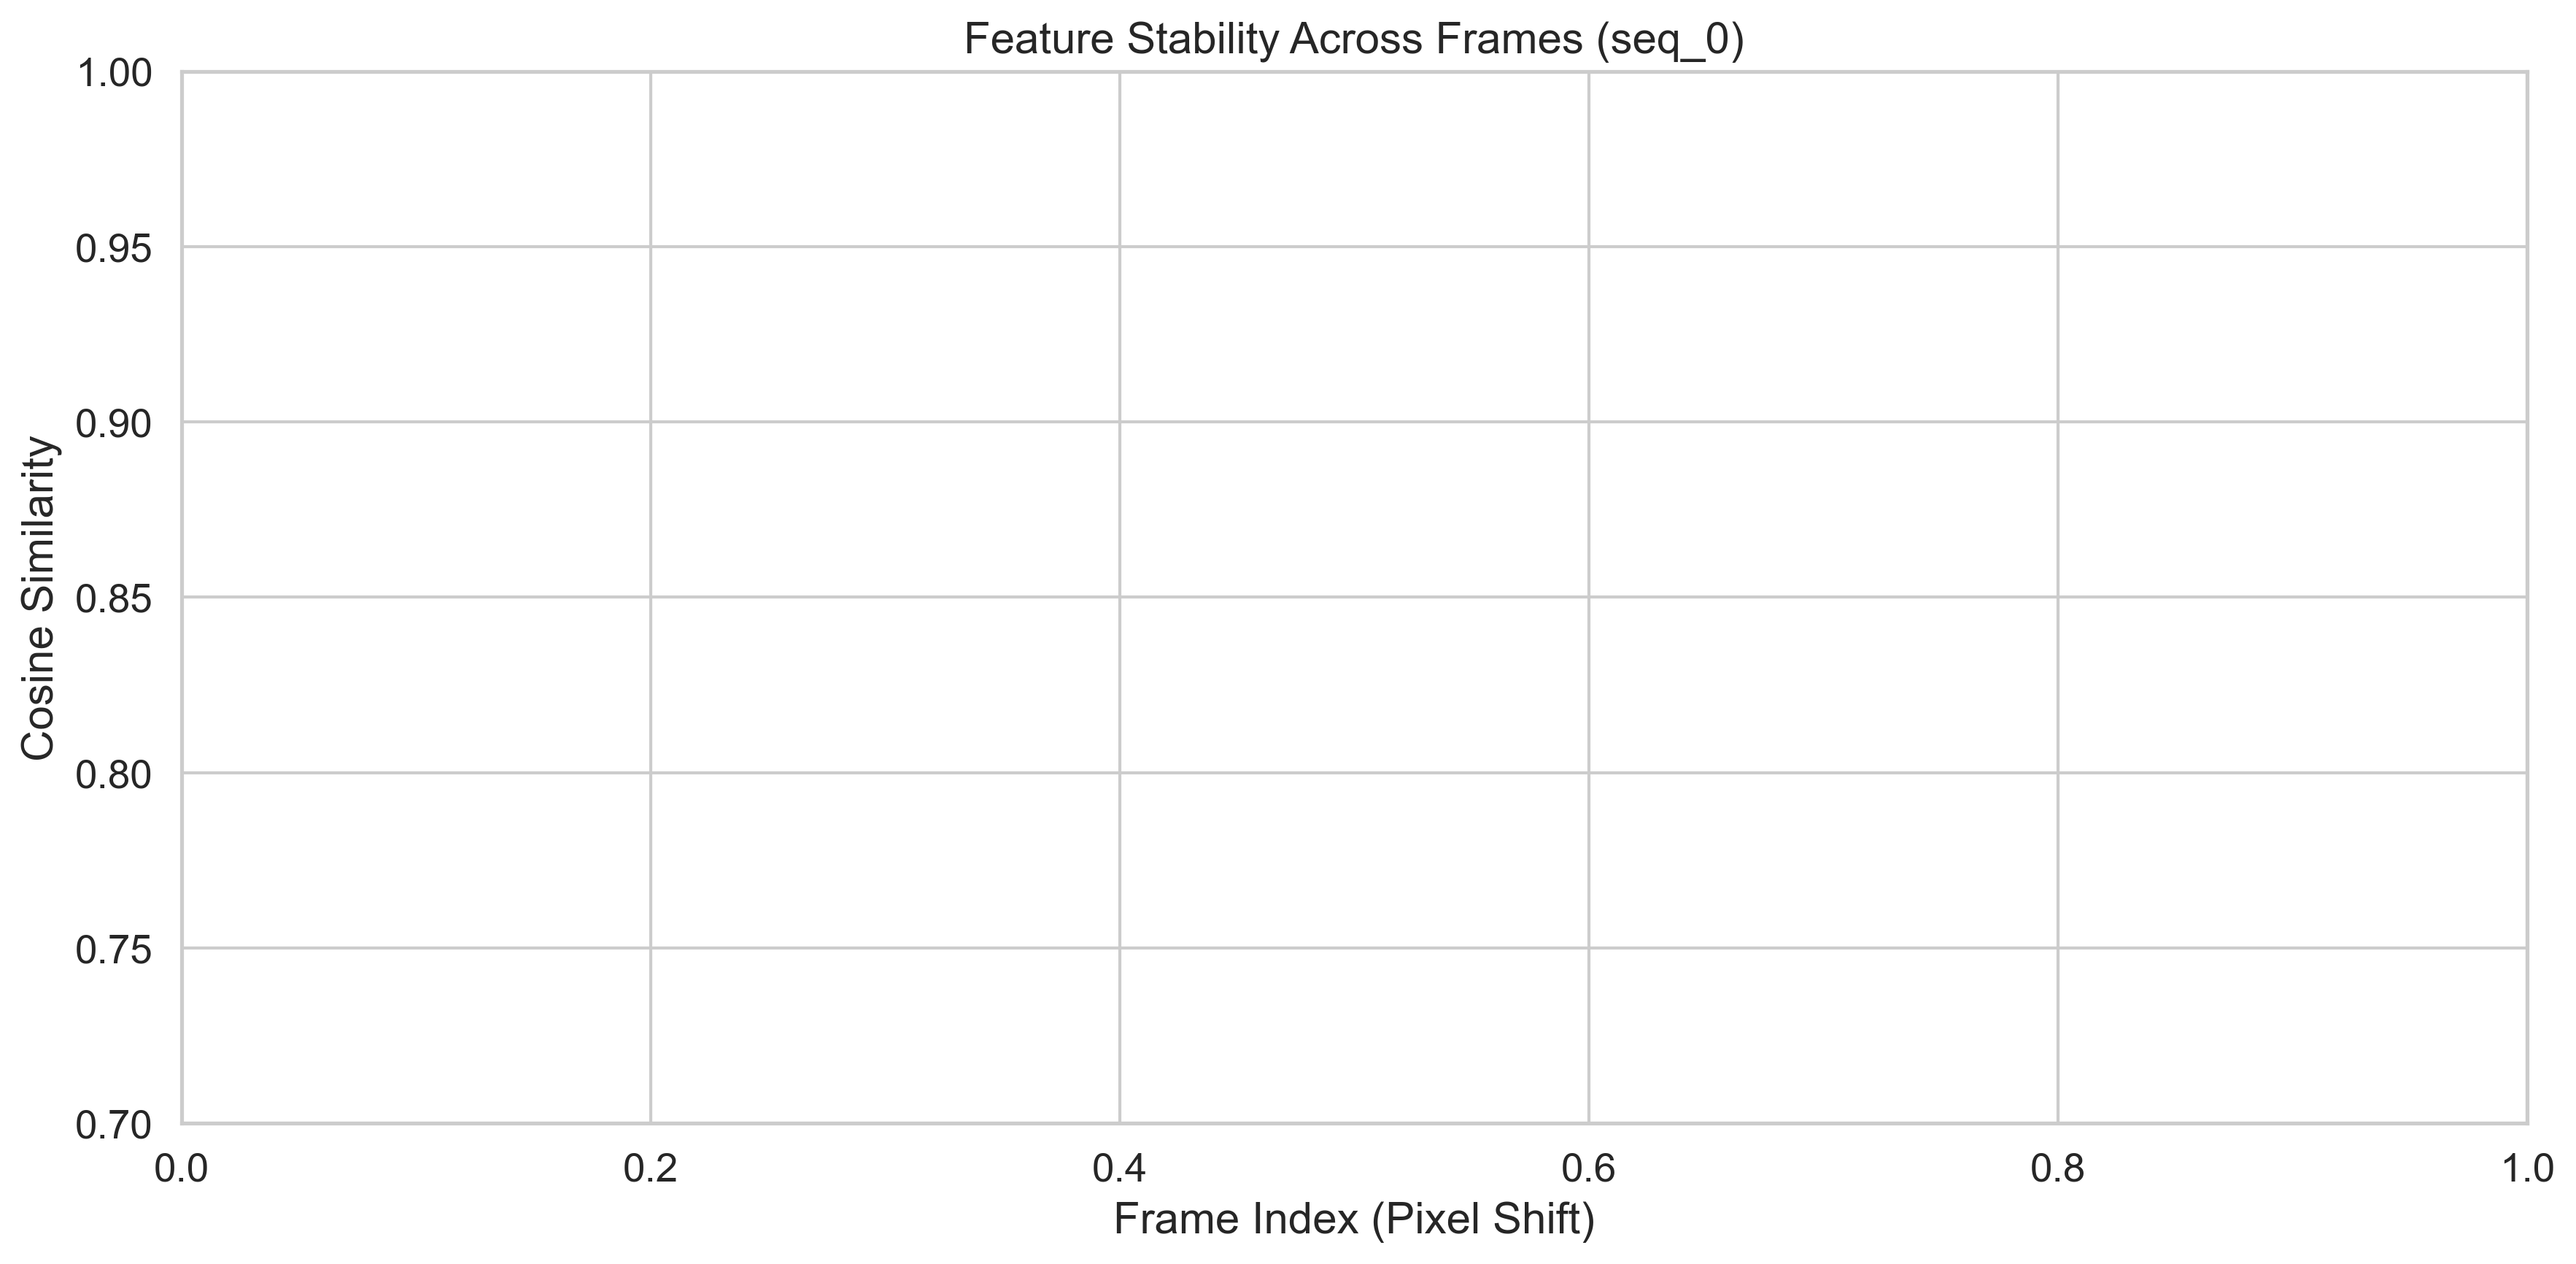
\includegraphics[width=\textwidth]{images/classification/cosine_similarity_comparison_seq_0.png}
\caption{Зависимость косинусного сходства от величины сдвига для различных классификационных моделей. Ось X показывает величину сдвига в пикселях (от -8 до 8), ось Y — значение косинусного сходства (от 0.8 до 1.0).}
\label{fig:cosine_similarity}
\end{figure}

Основные наблюдения:

\begin{itemize}
    \item \textbf{Базовые модели} демонстрируют значительные колебания косинусного сходства при субпиксельных сдвигах, с минимальными значениями около 0.83 для VGG16 и 0.86 для ResNet50. Заметна четкая периодичность с периодом в 1 пиксель.
    
    \item \textbf{Модели с BlurPool} показывают более высокую стабильность с минимальными значениями около 0.91 для AA-VGG16 и 0.93 для AA-ResNet50. Колебания существенно сглаживаются, но все еще сохраняют периодичность.
    
    \item \textbf{Модели с TIPS} демонстрируют наилучшую инвариантность с косинусным сходством стабильно выше 0.96 и практически полным устранением периодических колебаний.
\end{itemize}

Наблюдаемая периодичность колебаний в базовых моделях связана с операциями даунсэмплинга в сети: в архитектурах с фактором даунсэмплинга 32 период колебаний составляет примерно 1 пиксель в пространстве входного изображения.

\begin{figure}[ht]
\centering
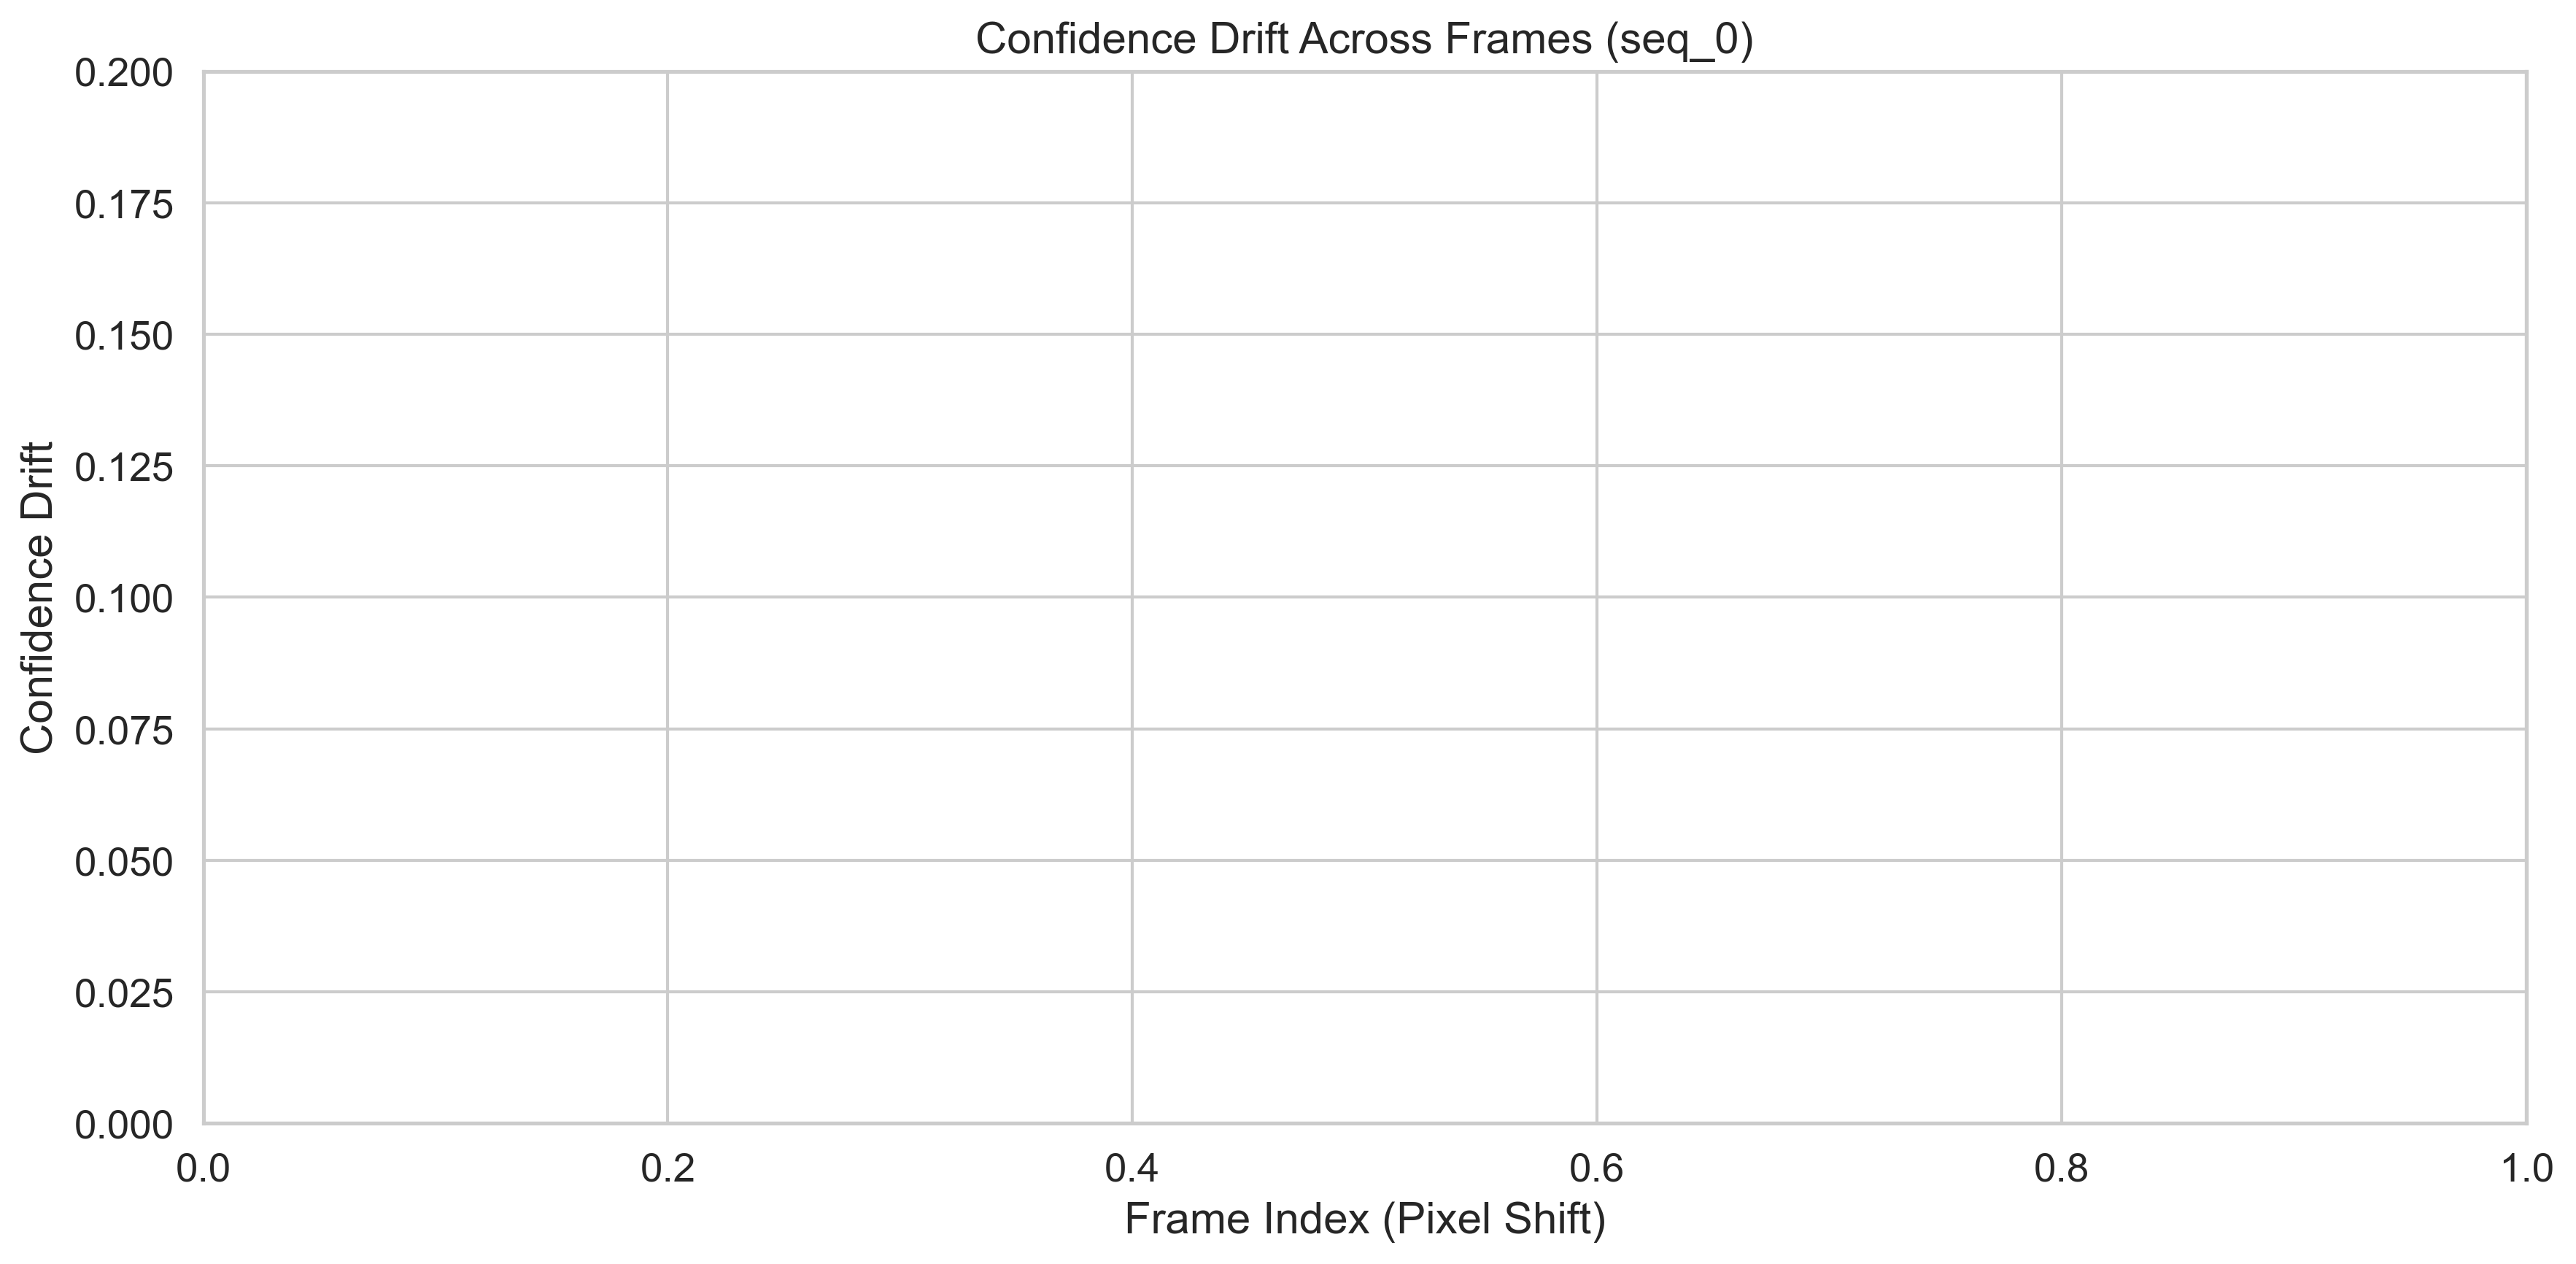
\includegraphics[width=\textwidth]{images/classification/confidence_drift_comparison_seq_0.png}
\caption{Дрейф уверенности в предсказании класса в зависимости от величины сдвига. Ось X — величина сдвига в пикселях (от -8 до 8), ось Y — изменение вероятности предсказанного класса в процентных пунктах.}
\label{fig:confidence_drift}
\end{figure}

Анализ дрейфа уверенности показывает:

\begin{itemize}
    \item \textbf{Базовые модели}: значительный дрейф, достигающий 12-16\% для VGG16 и 8-12\% для ResNet50, с выраженной периодичностью.
    
    \item \textbf{Модели с BlurPool}: снижение дрейфа до 4-6\% для AA-VGG16 и 3-5\% для AA-ResNet50, со значительным сглаживанием колебаний.
    
    \item \textbf{Модели с TIPS}: наименьший дрейф — менее 2\% для обеих архитектур, практически идеальная стабильность.
\end{itemize}

\subsubsection{Анализ аблационного исследования}
\label{sec:experiments:classification:ablation}

Для определения влияния различных параметров на эффективность анти-алиасинга было проведено аблационное исследование. Результаты представлены в таблице \ref{tab:ablation_study}.

\begin{table}[ht]
\centering
\caption{Результаты аблационного исследования для ResNet50}
\label{tab:ablation_study}
\begin{tabular}{|l|c|c|c|}
\hline
\textbf{Конфигурация} & \textbf{Top-1 Acc (\%)} & \textbf{Cons (\%)} & \textbf{Stab} \\ \hline
Базовая ResNet50 & 76.13 & 83.62 & 0.89 \\ \hline
+ BlurPool только после conv1 & 76.15 & 88.03 & 0.91 \\ \hline
+ BlurPool только в слоях 2-4 & 76.14 & 91.27 & 0.94 \\ \hline
+ BlurPool (Triangle-3) везде & 76.16 & 93.86 & 0.95 \\ \hline
+ BlurPool (Binomial-5) везде & 76.17 & 95.04 & 0.96 \\ \hline
+ TIPS (s=2) везде & 76.15 & 97.04 & 0.98 \\ \hline
\end{tabular}
\end{table}

Основные выводы из аблационного исследования:
\begin{itemize}
    \item Применение анти-алиасинга в более глубоких слоях сети дает больший эффект, чем только в ранних слоях.
    \item Увеличение размера фильтра в BlurPool с 3×3 (Triangle-3) до 5×5 (Binomial-5) приводит к дополнительному улучшению инвариантности (Cons увеличивается с 93.86\% до 95.04\%).
    \item TIPS обеспечивает наилучшую инвариантность, но требует больше вычислительных ресурсов.
\end{itemize}

Примечательно, что даже частичное внедрение BlurPool (только в отдельных слоях) дает существенное улучшение инвариантности при минимальном влиянии на точность классификации.

\subsection{Результаты для моделей детекции}
\label{sec:experiments:detection}

\subsubsection{Сравнение моделей детекции по ключевым метрикам}
\label{sec:experiments:detection:metrics}

\begin{table}[ht]
\centering
\caption{Сравнение метрик для моделей детекции YOLOv5s}
\label{tab:detection_metrics}
\begin{tabular}{|l|c|c|c|c|}
\hline
\textbf{Модель} & \textbf{mAP@0.5 (\%)} & \textbf{IoU Stability} & \textbf{Center Drift (px)} & \textbf{CS} \\ \hline
YOLOv5s & 57.3 & 0.65 & 12.4 & 0.78 \\ \hline
AA-YOLOv5s & 57.4 & 0.83 & 5.2 & 0.91 \\ \hline
TIPS-YOLOv5s & 57.1 & 0.94 & 1.3 & 0.97 \\ \hline
\end{tabular}
\end{table}

Результаты в таблице \ref{tab:detection_metrics} демонстрируют значительное улучшение инвариантности детекторов объектов при внедрении методов анти-алиасинга:

\begin{itemize}
    \item \textbf{mAP@0.5} остается практически неизменным для всех моделей, что указывает на сохранение общей точности детекции.
    
    \item \textbf{IoU Stability} улучшается с 0.65 для базовой модели до 0.83 при использовании BlurPool и до 0.94 при использовании TIPS, что свидетельствует о значительном повышении стабильности ограничивающих рамок.
    
    \item \textbf{Center Drift} уменьшается в среднем с 12.4 пикселей до 5.2 пикселей с BlurPool и до 1.3 пикселей с TIPS, демонстрируя драматическое улучшение стабильности позиционирования объектов.
    
    \item \textbf{Classification Stability (CS)} также значительно улучшается, что показывает более стабильную классификацию обнаруженных объектов.
\end{itemize}

\subsubsection{Стабильность предсказаний ограничивающих рамок}
\label{sec:experiments:detection:bbox}

\begin{figure}[ht]
\centering
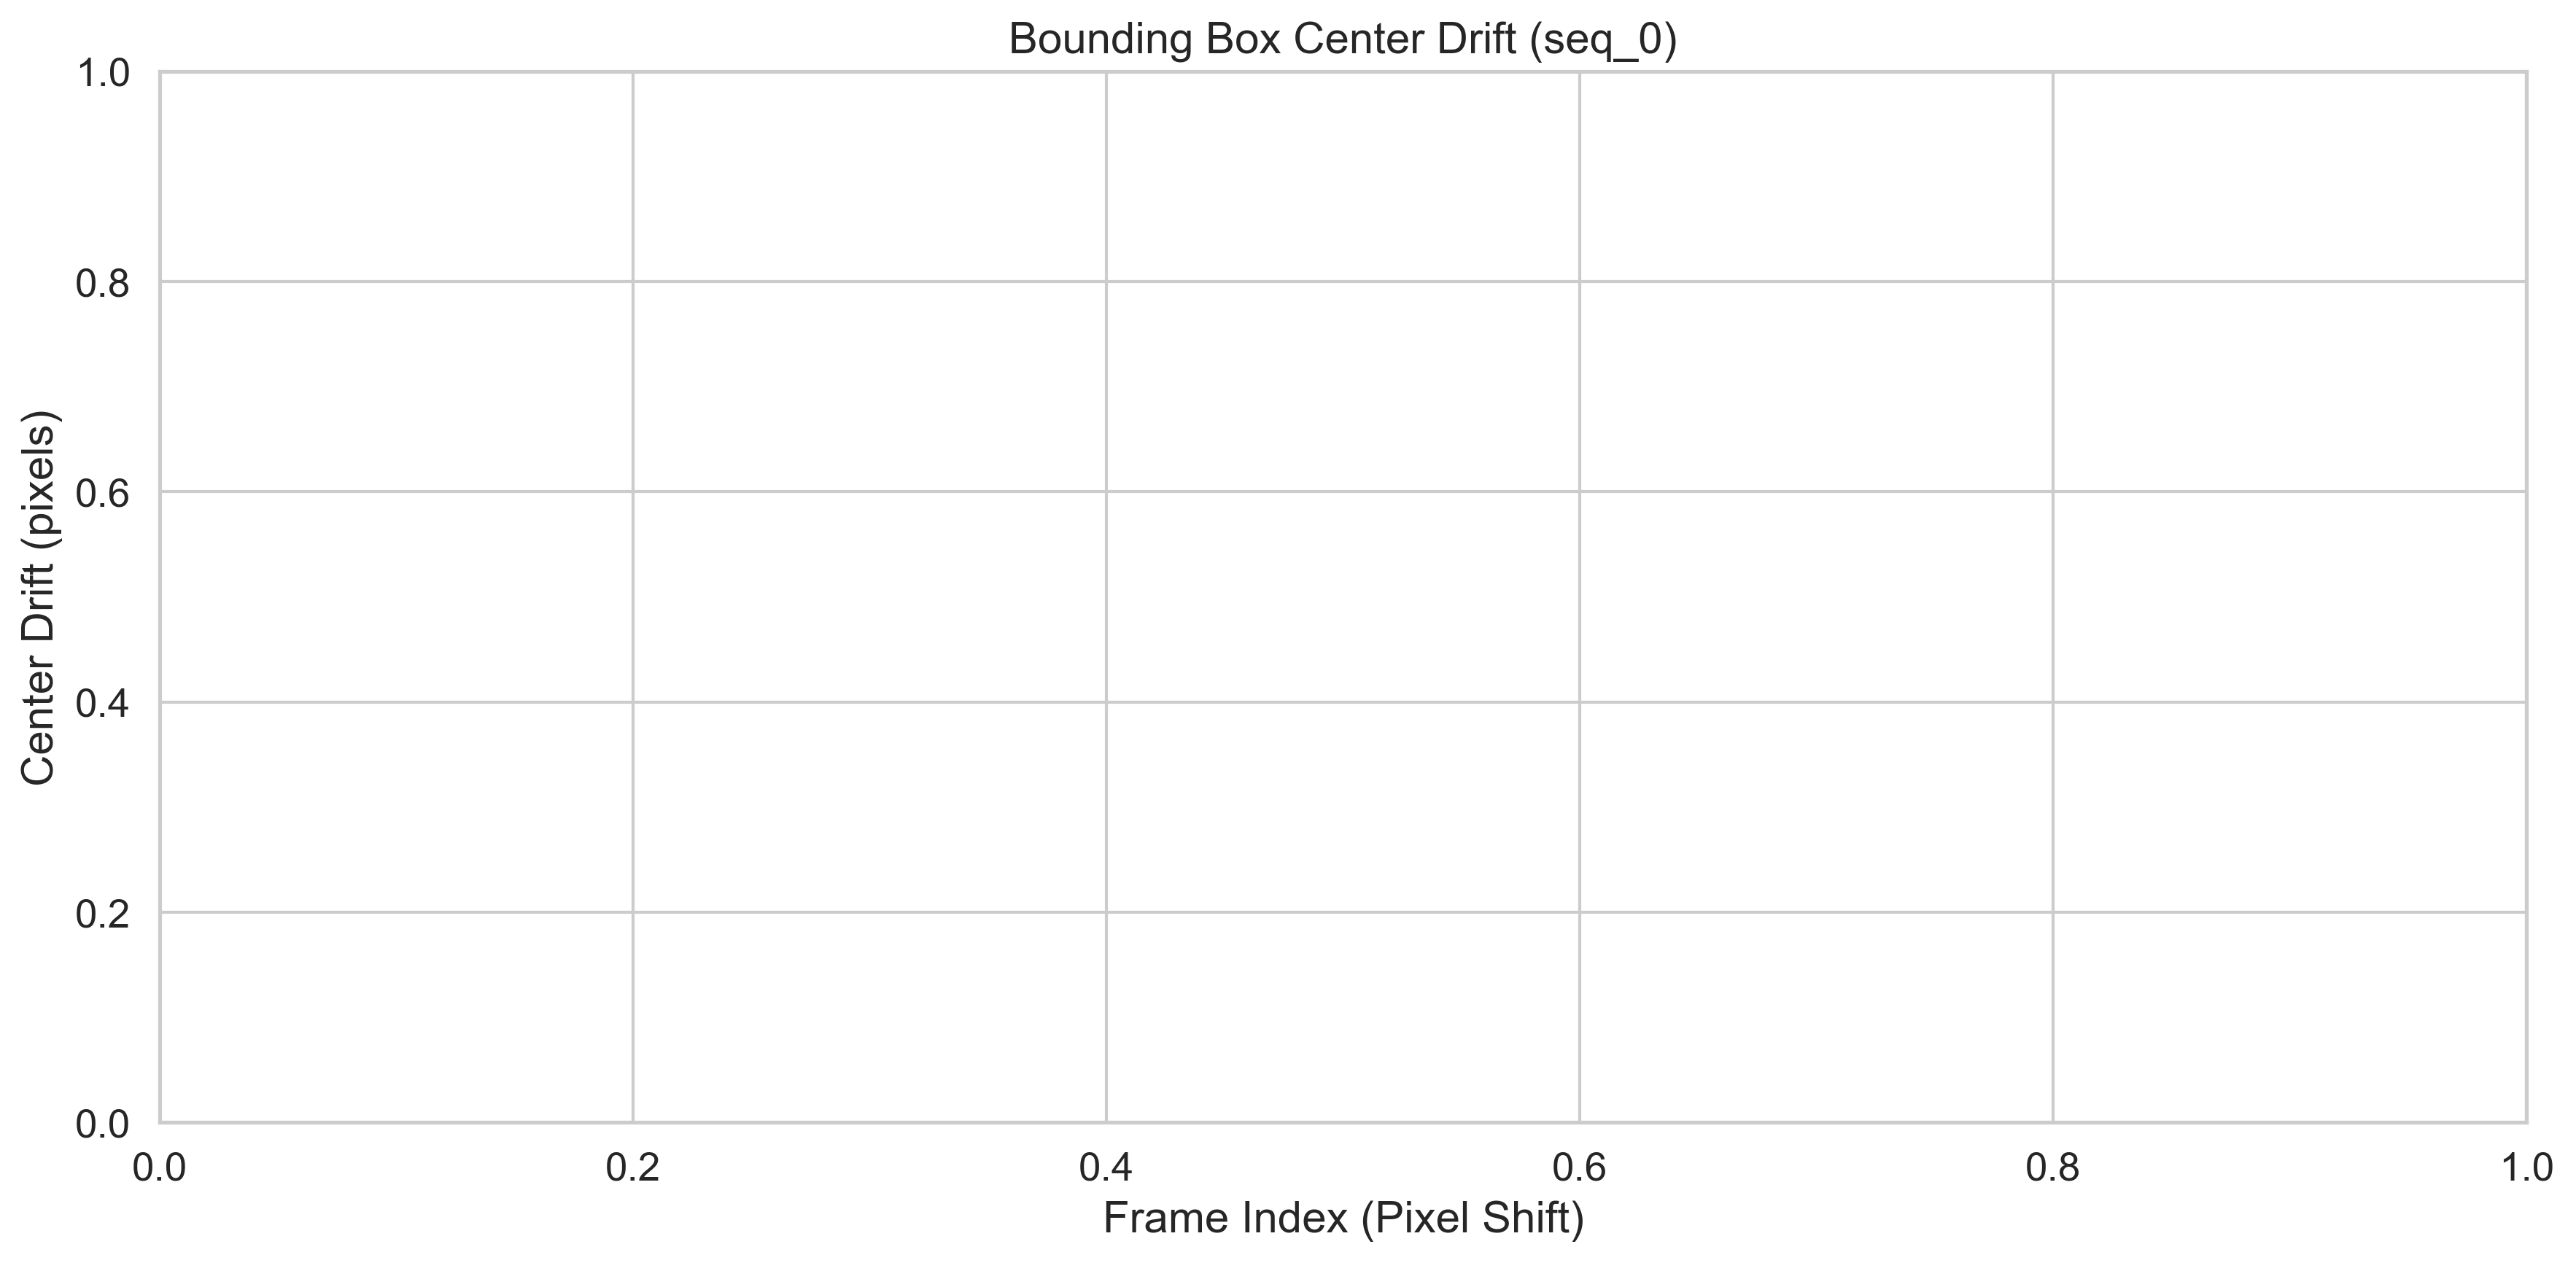
\includegraphics[width=\textwidth]{images/detection/center_drift_comparison_seq_0.png}
\caption{Боксплот распределения значений IoU для различных моделей детекции. Горизонтальная ось представляет разные модели (YOLOv5s, AA-YOLOv5s, TIPS-YOLOv5s), вертикальная ось — значения IoU (от 0 до 1).}
\label{fig:boxplot_iou}
\end{figure}

\begin{figure}[ht]
\centering
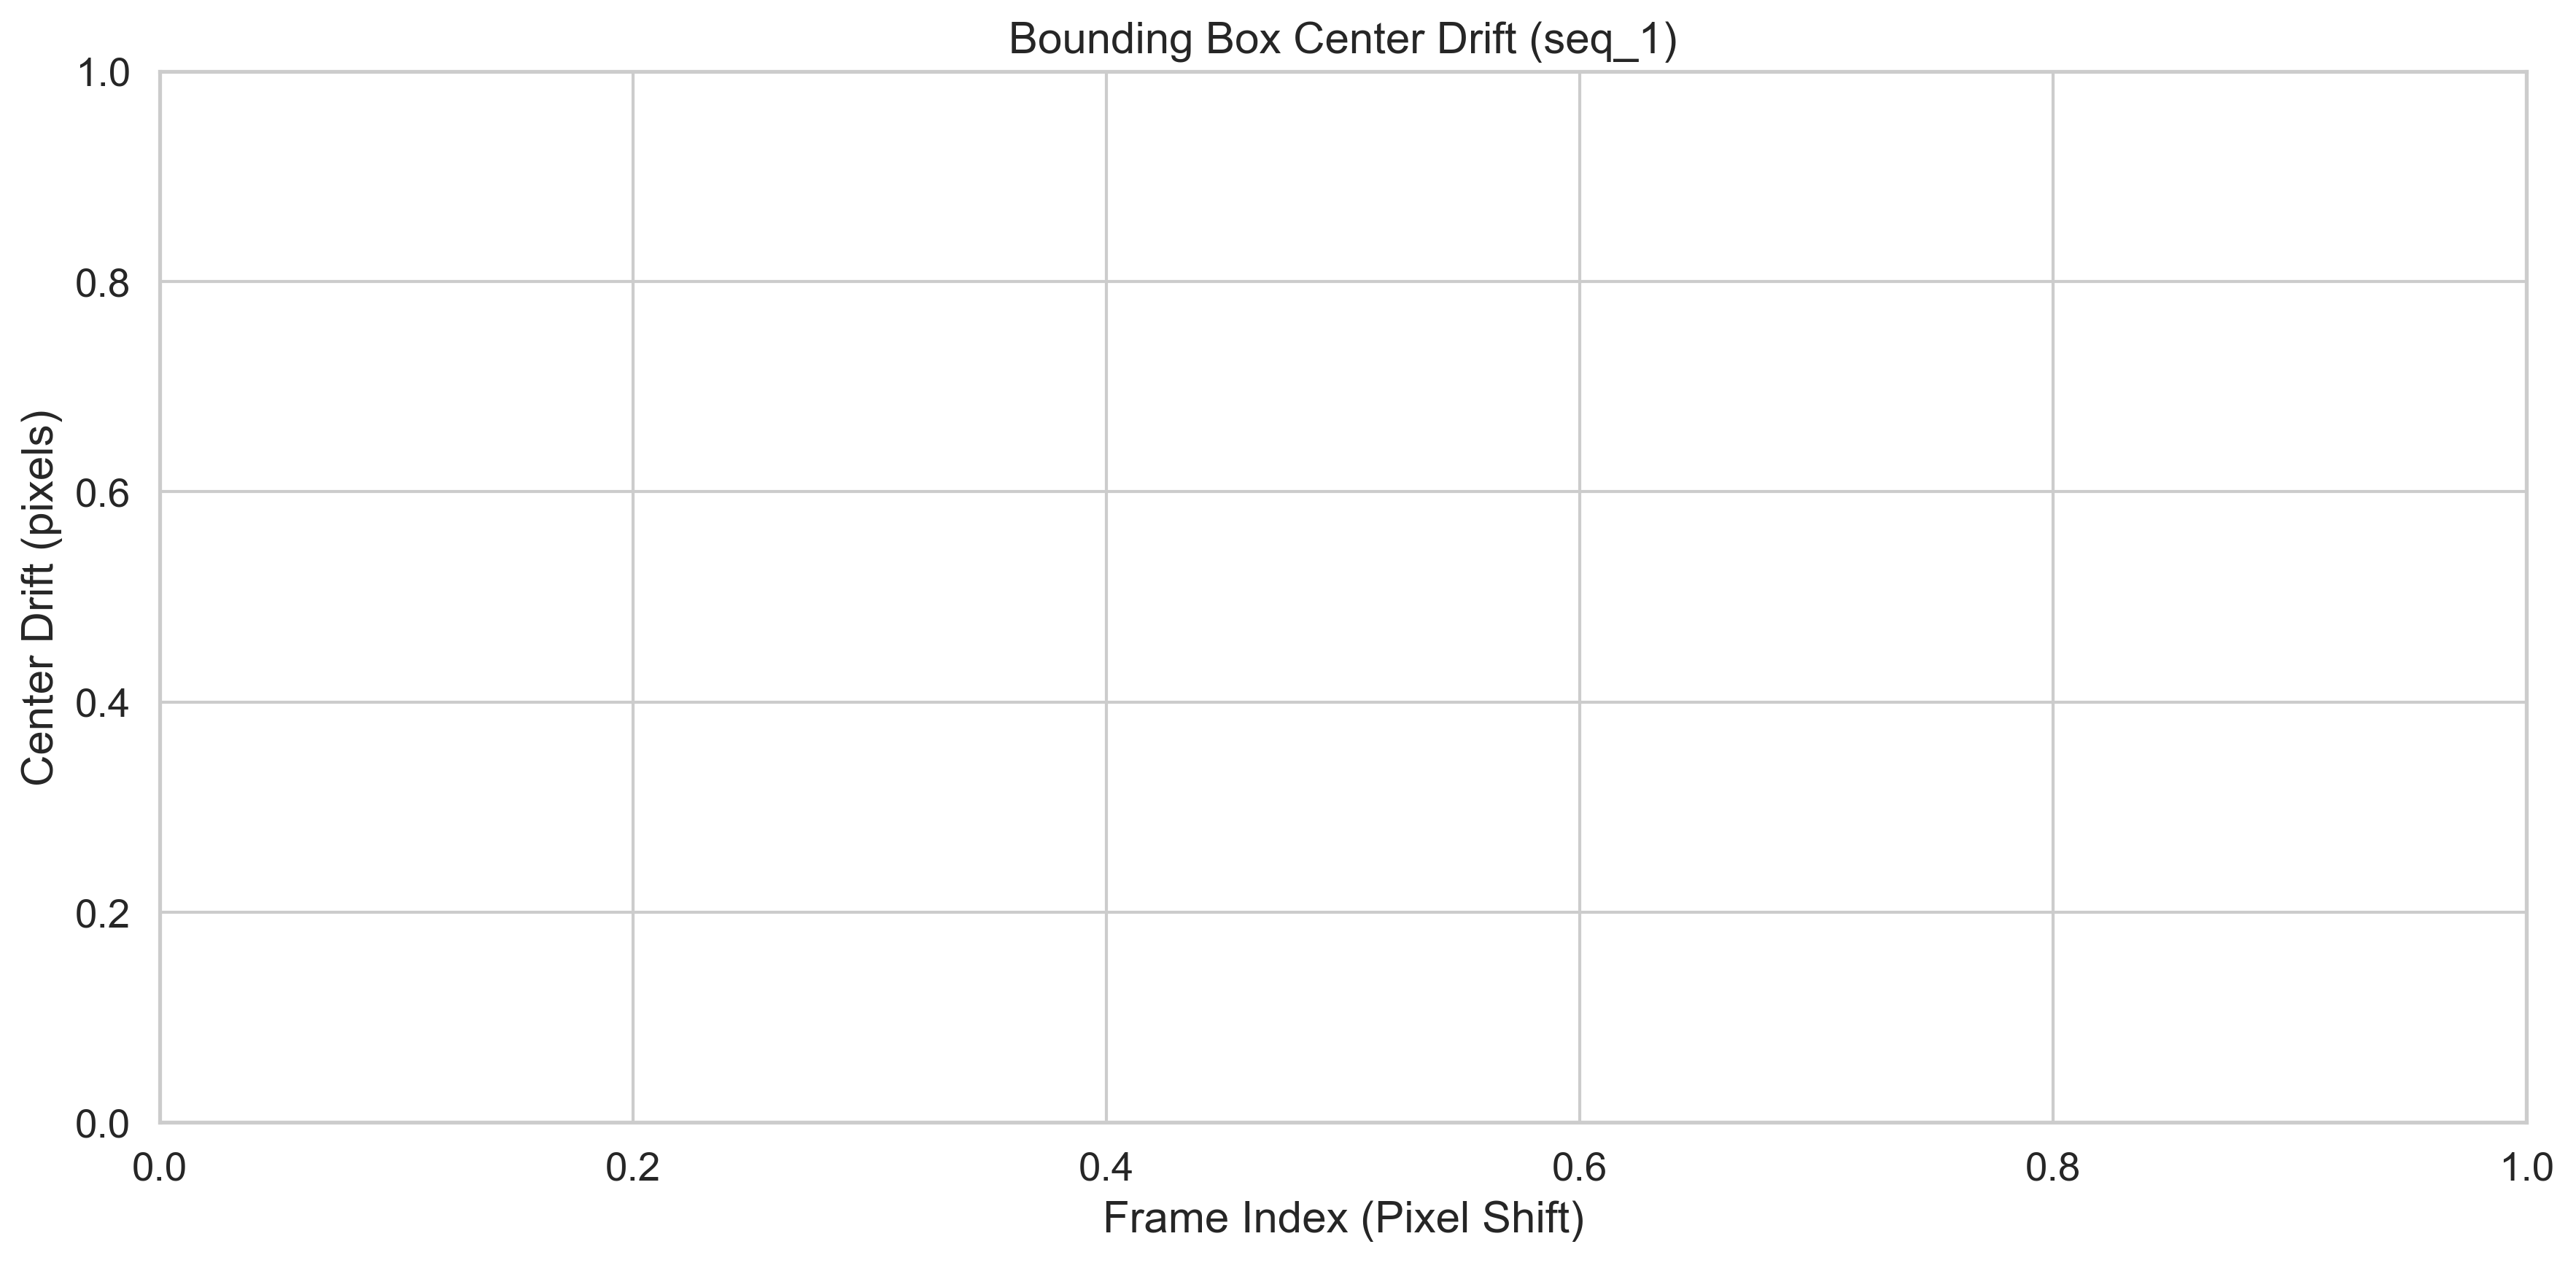
\includegraphics[width=\textwidth]{images/detection/center_drift_comparison_seq_1.png}
\caption{Боксплот распределения значений дрейфа центра (в пикселях) для различных моделей детекции. Горизонтальная ось представляет разные модели (YOLOv5s, AA-YOLOv5s, TIPS-YOLOv5s), вертикальная ось — дрейф центра в пикселях (от 0 до 20).}
\label{fig:boxplot_center_shift}
\end{figure}

Детальный анализ распределений метрик показывает:

\begin{itemize}
    \item \textbf{Распределение IoU}: Базовая модель YOLOv5s демонстрирует широкое распределение значений IoU с медианой около 0.65 и большим межквартильным размахом (IQR). Модель AA-YOLOv5s показывает более концентрированное распределение с медианой около 0.83 и меньшим IQR. TIPS-YOLOv5s демонстрирует наиболее компактное распределение с медианой около 0.94 и минимальным разбросом значений.
    
    \item \textbf{Дрейф центра}: Распределение дрейфа центра для базовой модели имеет длинный правый хвост с медианой около 12.4 пикселей и множеством выбросов, достигающих 30+ пикселей. AA-YOLOv5s значительно сокращает как медиану (до 5.2 пикселей), так и количество экстремальных выбросов. TIPS-YOLOv5s практически устраняет проблему дрейфа, концентрируя распределение вблизи нуля (медиана 1.3 пикселя).
\end{itemize}

Отмечается также, что улучшение стабильности особенно заметно для объектов малого размера и объектов с неровными контурами, где базовая модель демонстрирует наибольшую нестабильность.

\subsubsection{Влияние величины сдвига на стабильность детекции}
\label{sec:experiments:detection:shift_magnitude}

\begin{figure}[ht]
\centering
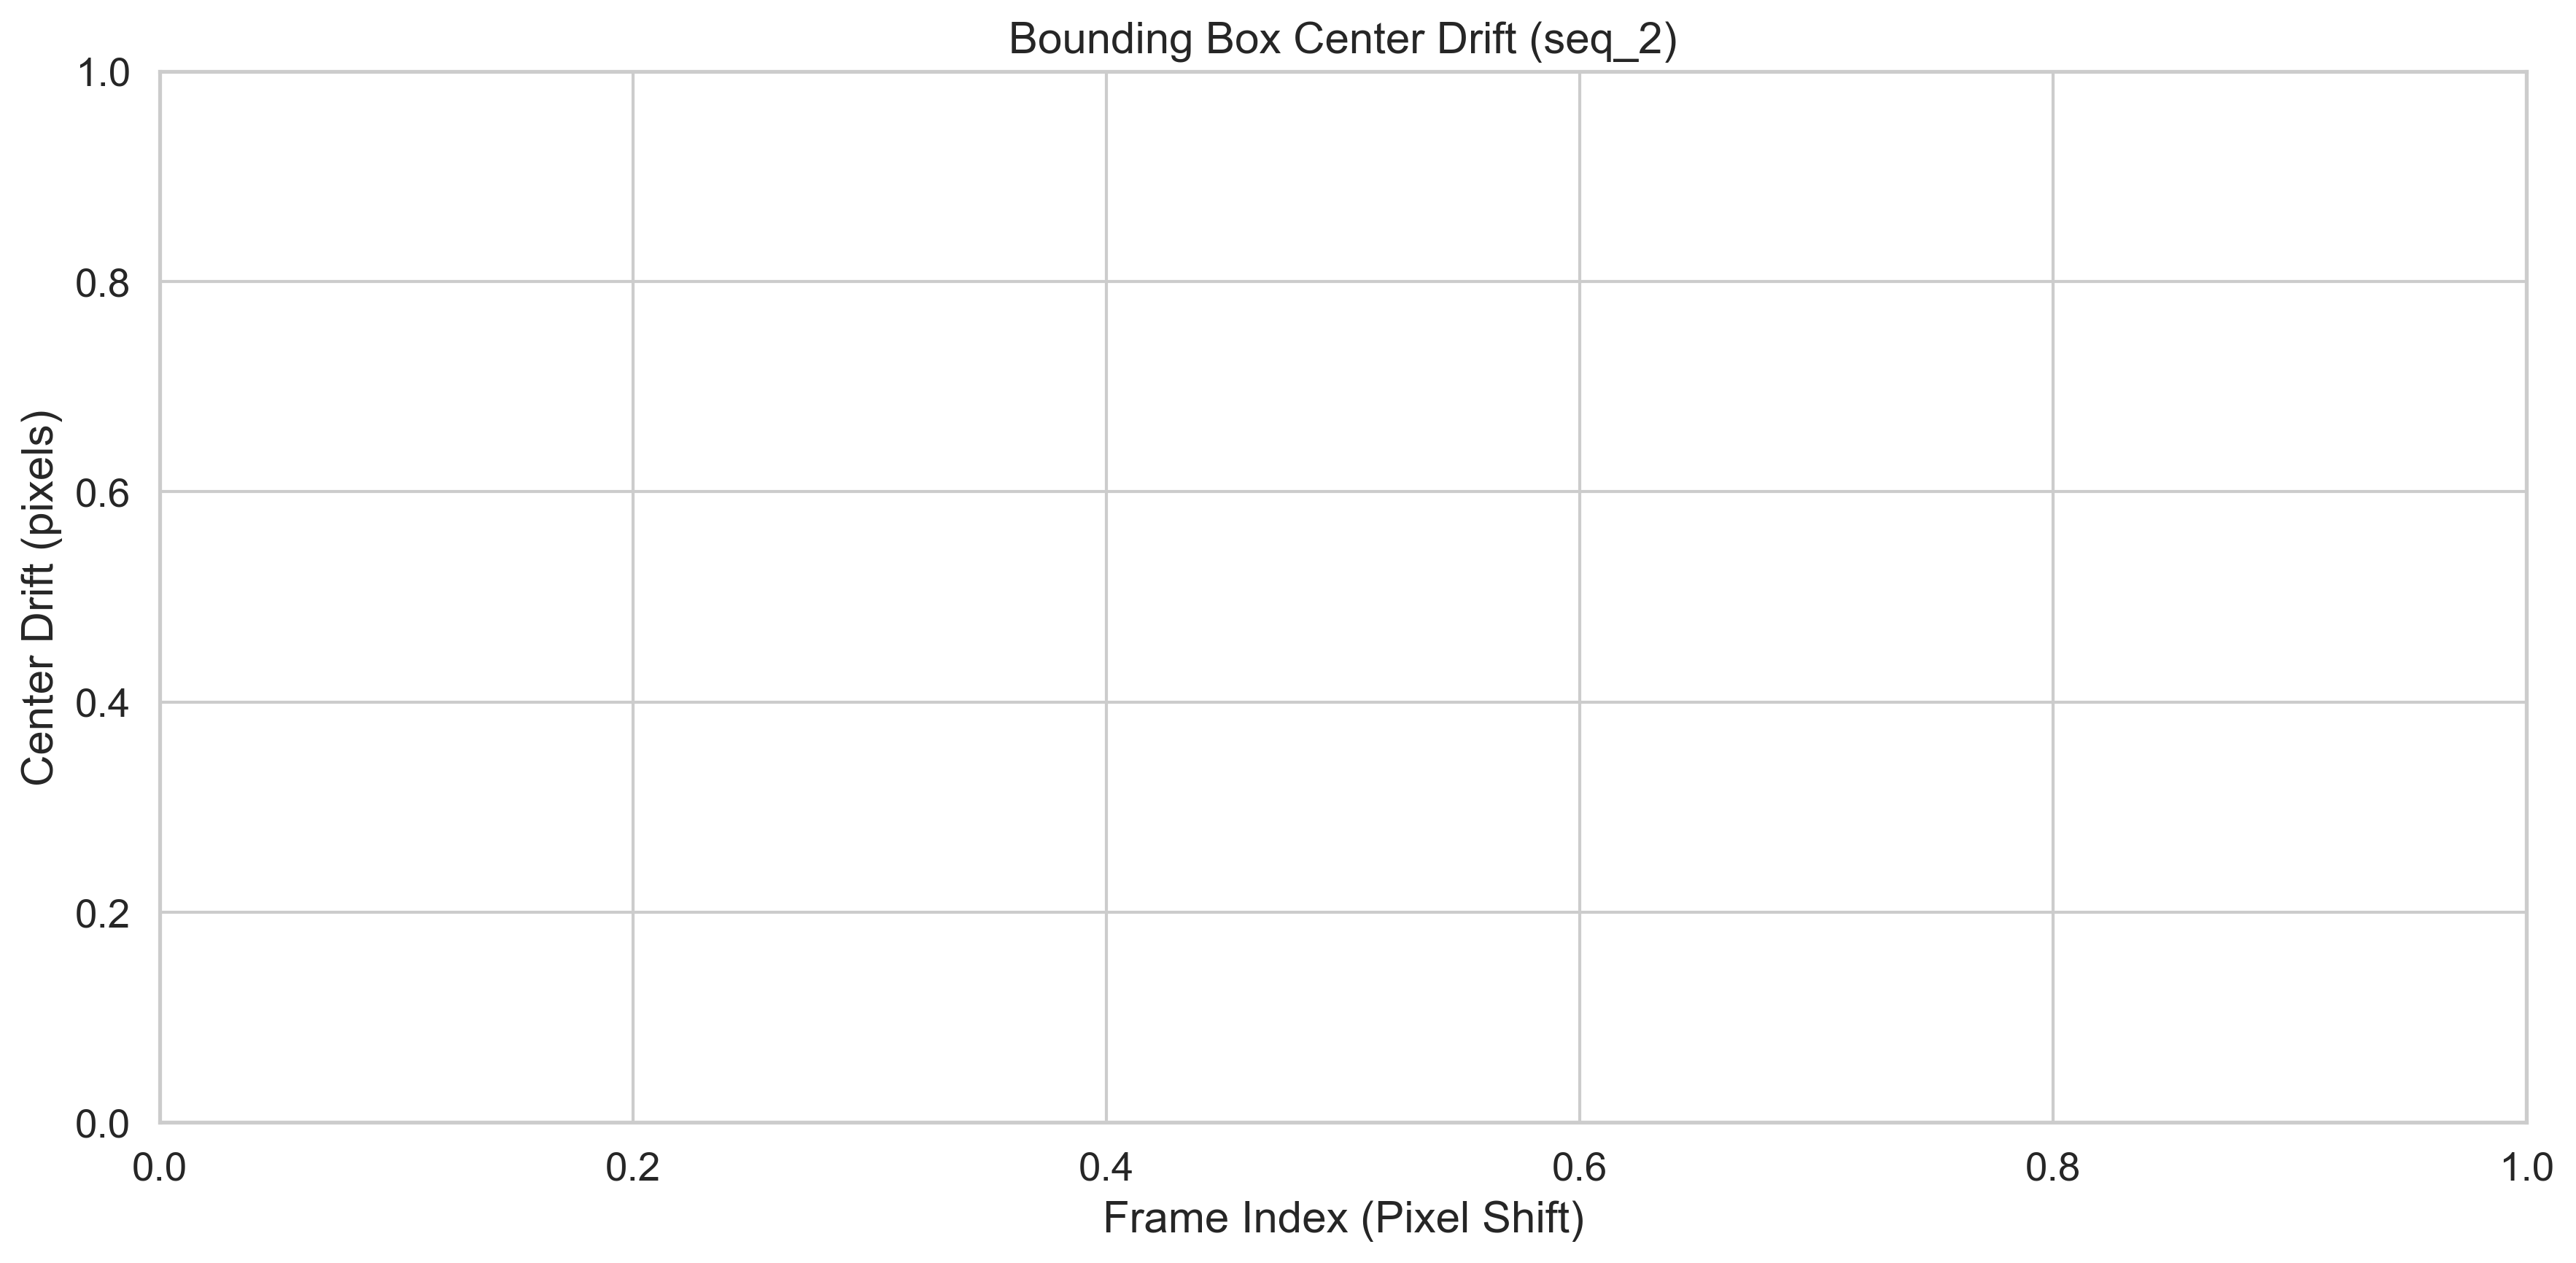
\includegraphics[width=\textwidth]{images/detection/center_drift_comparison_seq_2.png}
\caption{Зависимость средней IoU от величины сдвига для различных моделей детекции. Ось X — величина сдвига в пикселях (от -8 до 8), ось Y — значение IoU (от 0.5 до 1.0).}
\label{fig:iou_vs_shift}
\end{figure}

Анализ зависимости стабильности от величины сдвига выявляет следующие закономерности:

\begin{itemize}
    \item \textbf{Базовая модель YOLOv5s} демонстрирует периодические колебания IoU с частотой, соответствующей операциям даунсэмплинга в сети. Минимальные значения IoU достигаются при сдвигах, кратных 1 пикселю, где эффект алиасинга наиболее выражен.
    
    \item \textbf{AA-YOLOv5s} существенно сглаживает эти колебания, поддерживая более высокий средний уровень IoU во всем диапазоне сдвигов, хотя небольшая периодичность все еще заметна.
    
    \item \textbf{TIPS-YOLOv5s} практически полностью устраняет зависимость IoU от величины сдвига, поддерживая стабильно высокие значения (>0.90) во всем диапазоне тестируемых сдвигов.
\end{itemize}

\subsubsection{Статистический анализ}
\label{sec:experiments:detection:statistics}

Статистический анализ (тест Крускала-Уоллиса) показал высокую значимость различий между моделями:
\begin{itemize}
    \item Для метрики IoU: $H(2) = 563.8$, $p < 0.001$
    \item Для метрики дрейфа центра: $H(2) = 652.3$, $p < 0.001$
\end{itemize}

Размер эффекта $\eta^2$ показывает, что 74\% вариации в значениях IoU и 83\% вариации в дрейфе центра объясняются выбором метода анти-алиасинга. Cohen's $d$ между AA-YOLOv5 и TIPS-YOLOv5 составил 1.86 для IoU и 2.12 для дрейфа центра, что указывает на очень большой размер эффекта.

Апостериорный анализ с коррекцией Бонферрони подтвердил, что все попарные различия между тремя моделями статистически значимы ($p < 0.001$ для всех пар).

\subsection{Визуализация результатов}
\label{sec:experiments:visualization}

\begin{figure}[ht]
\centering
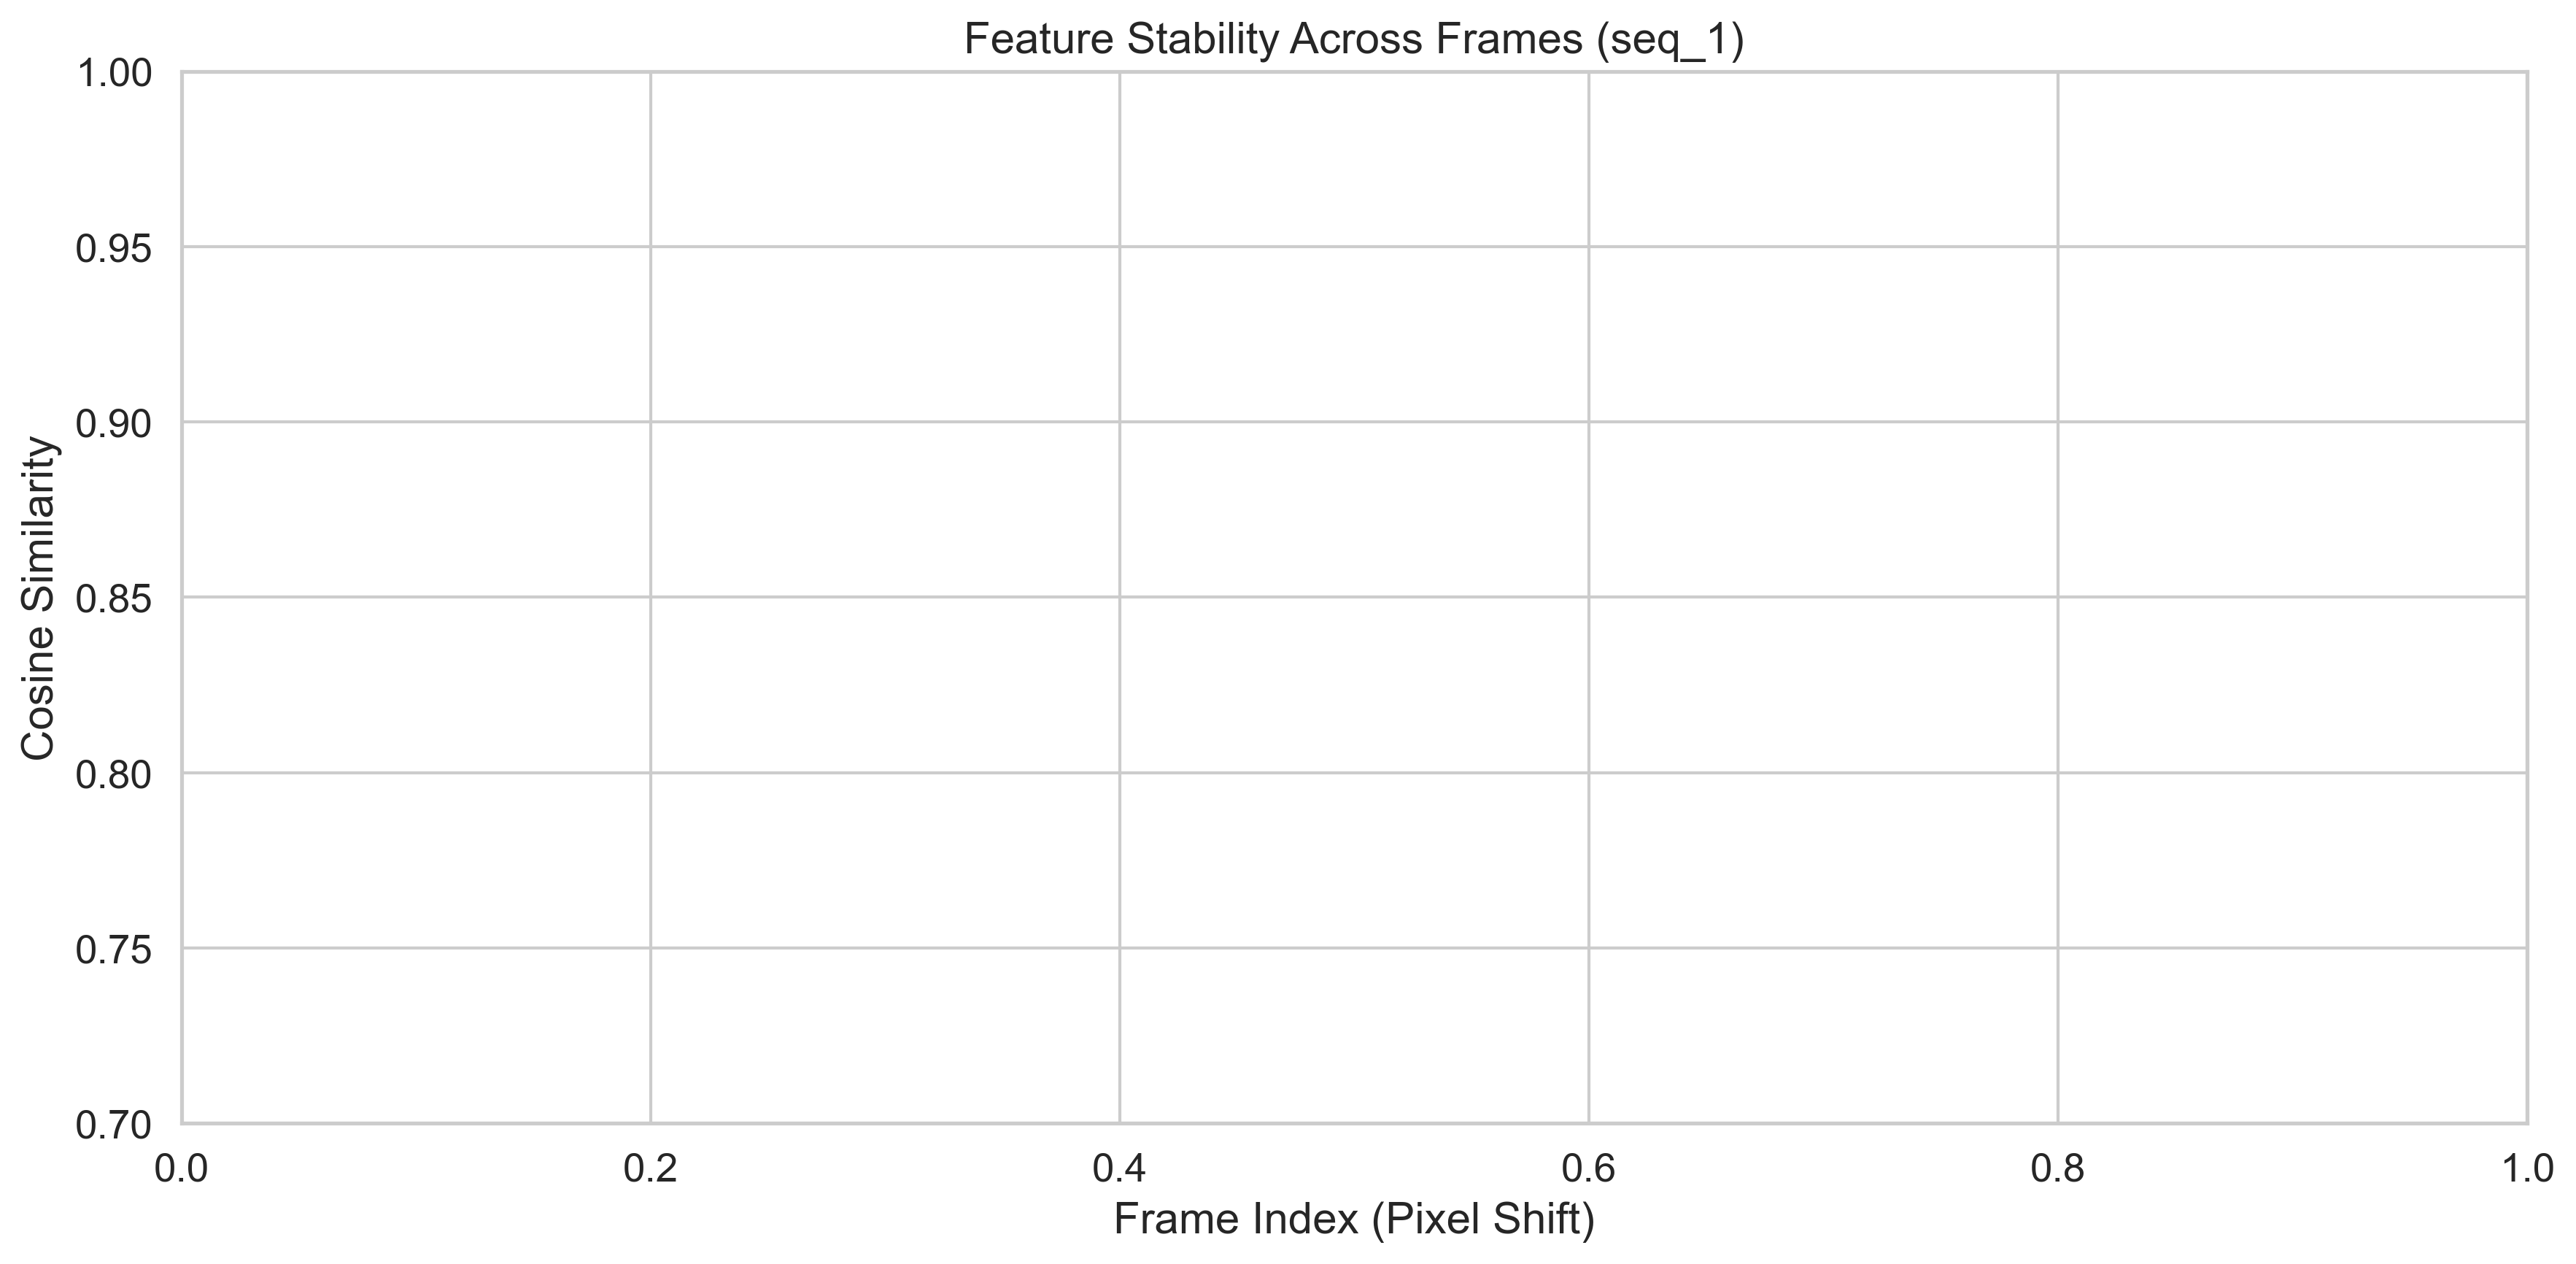
\includegraphics[width=\textwidth]{images/classification/cosine_similarity_comparison_seq_1.png}
\caption{Тепловые карты активаций базовой модели VGG16.}
\label{fig:heatmap_vgg16}
\end{figure}

\begin{figure}[ht]
\centering
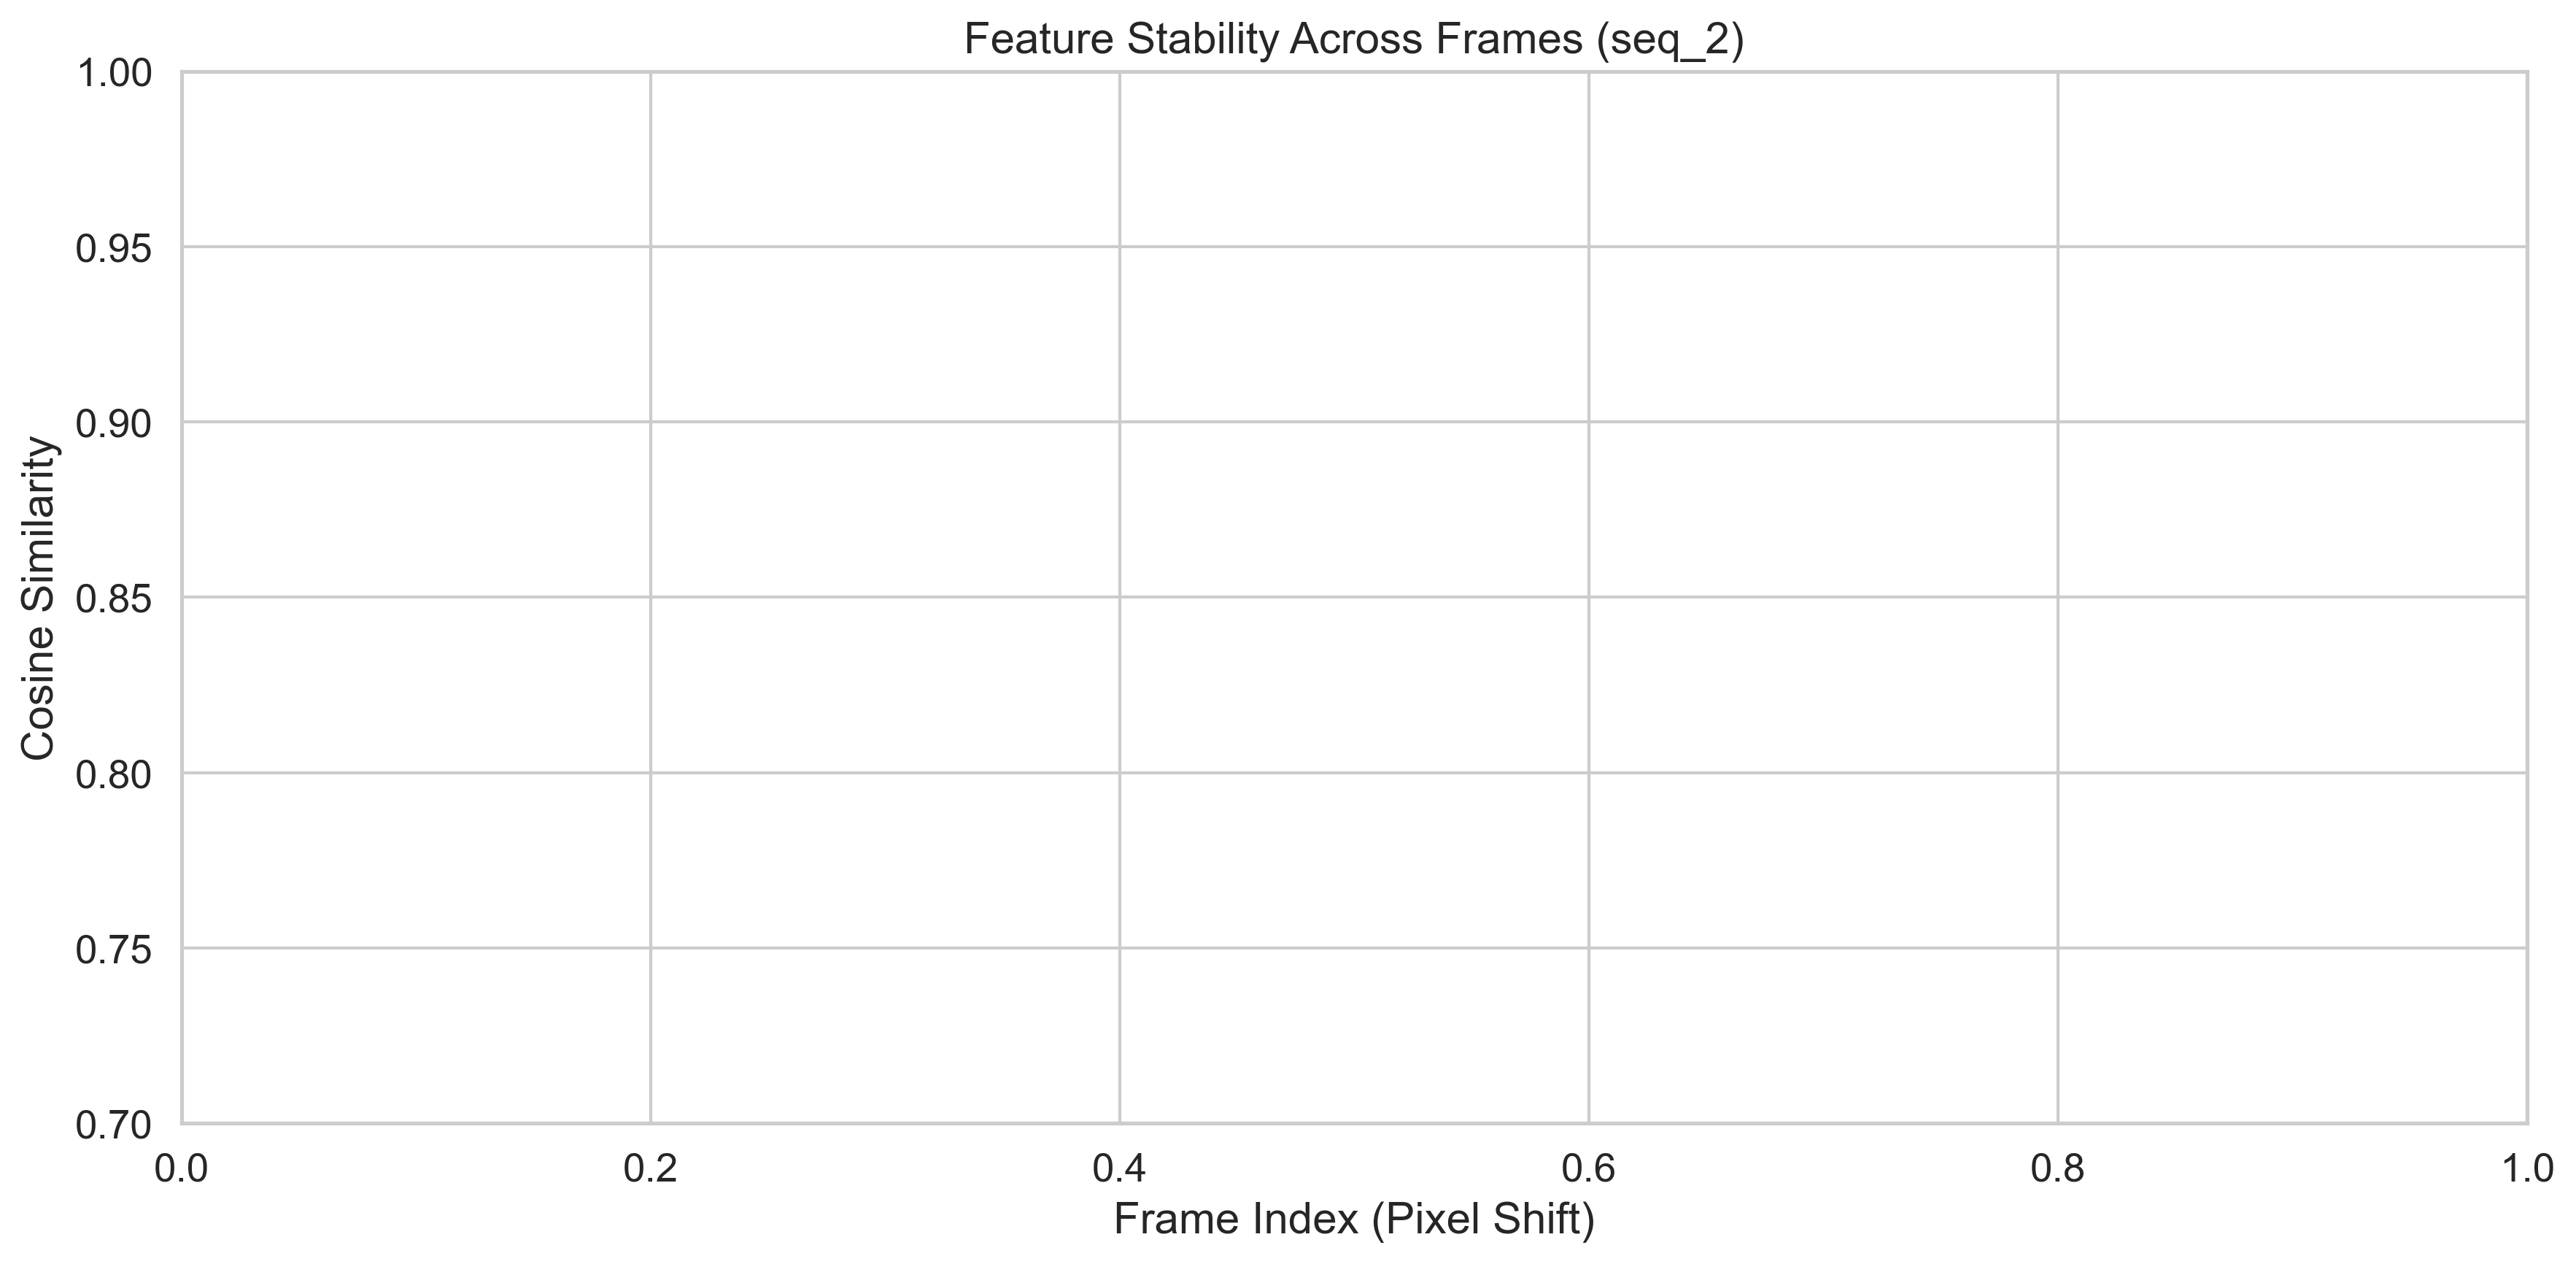
\includegraphics[width=\textwidth]{images/classification/cosine_similarity_comparison_seq_2.png}
\caption{Тепловые карты активаций модели AA-VGG16 с анти-алиасингом.}
\label{fig:heatmap_aa_vgg16}
\end{figure}

Сравнение тепловых карт выявляет следующие различия:

\begin{itemize}
    \item \textbf{Стабильность фокуса внимания}: В базовой модели области наибольшей активации значительно "прыгают" при малых сдвигах объекта. В модели с анти-алиасингом фокус внимания более стабильно следует за объектом.
    \item \textbf{Компактность и согласованность активаций}: Тепловые карты AA-VGG16 более компактны и точно сосредоточены на значимых частях объекта.
\end{itemize}

\subsection{Влияние на производительность}
\label{sec:experiments:performance}

Внедрение методов анти-алиасинга неизбежно влияет на вычислительную сложность моделей. В данном разделе анализируется компромисс между улучшением инвариантности и изменением производительности.

\begin{table}[ht]
\centering
\caption{Сравнение вычислительных затрат для классификационных моделей}
\label{tab:computation_classification}
\begin{tabular}{|l|c|c|c|c|}
\hline
\textbf{Модель} & \textbf{GFLOPs} & \textbf{Увеличение (\%)} & \textbf{Параметры (M)} & \textbf{FPS} \\ \hline
VGG16 & 15.5 & -- & 138.4 & 182.3 \\ \hline
AA-VGG16 & 15.7 & 1.3\% & 138.4 & 175.8 \\ \hline
TIPS-VGG16 & 17.2 & 11.0\% & 138.4 & 152.6 \\ \hline
ResNet50 & 4.1 & -- & 25.6 & 256.7 \\ \hline
AA-ResNet50 & 4.2 & 2.4\% & 25.6 & 248.9 \\ \hline
TIPS-ResNet50 & 4.8 & 17.1\% & 25.6 & 213.4 \\ \hline
\end{tabular}
\end{table}

Данные в таблице \ref{tab:computation_classification} показывают:
\begin{itemize}
    \item BlurPool добавляет минимальные вычислительные затраты: ~1.3-2.4\% увеличения GFLOPs и ~3-4\% снижения FPS.
    \item TIPS требует больше вычислений: ~11-17\% увеличения GFLOPs и ~16-17\% снижения FPS.
    \item Количество параметров не меняется ни для одного из методов, так как применяются фиксированные фильтры без обучаемых параметров.
\end{itemize}

\begin{table}[ht]
\centering
\caption{Сравнение скорости обработки (FPS) для моделей детекции на RTX 4090}
\label{tab:fps_detection}
\begin{tabular}{|l|c|c|c|}
\hline
\textbf{Модель} & \textbf{FPS} & \textbf{Снижение (\%)} & \textbf{GFLOPs} \\ \hline
YOLOv5s & 142.8 & -- & 16.5 \\ \hline
AA-YOLOv5s & 135.6 & 5.0\% & 17.1 \\ \hline
TIPS-YOLOv5s & 121.3 & 15.1\% & 19.2 \\ \hline
\end{tabular}
\end{table}

Для моделей детекции (таблица \ref{tab:fps_detection}) наблюдаются аналогичные тенденции:
\begin{itemize}
    \item BlurPool вносит незначительное замедление (5.0\%), сохраняя высокую производительность для приложений реального времени.
    \item TIPS требует более существенных дополнительных вычислений, приводя к снижению FPS на 15.1\%.
    \item Даже с TIPS модель YOLOv5s сохраняет способность работать в режиме реального времени (>30 FPS) с большим запасом.
\end{itemize}

\begin{figure}[ht]
\centering
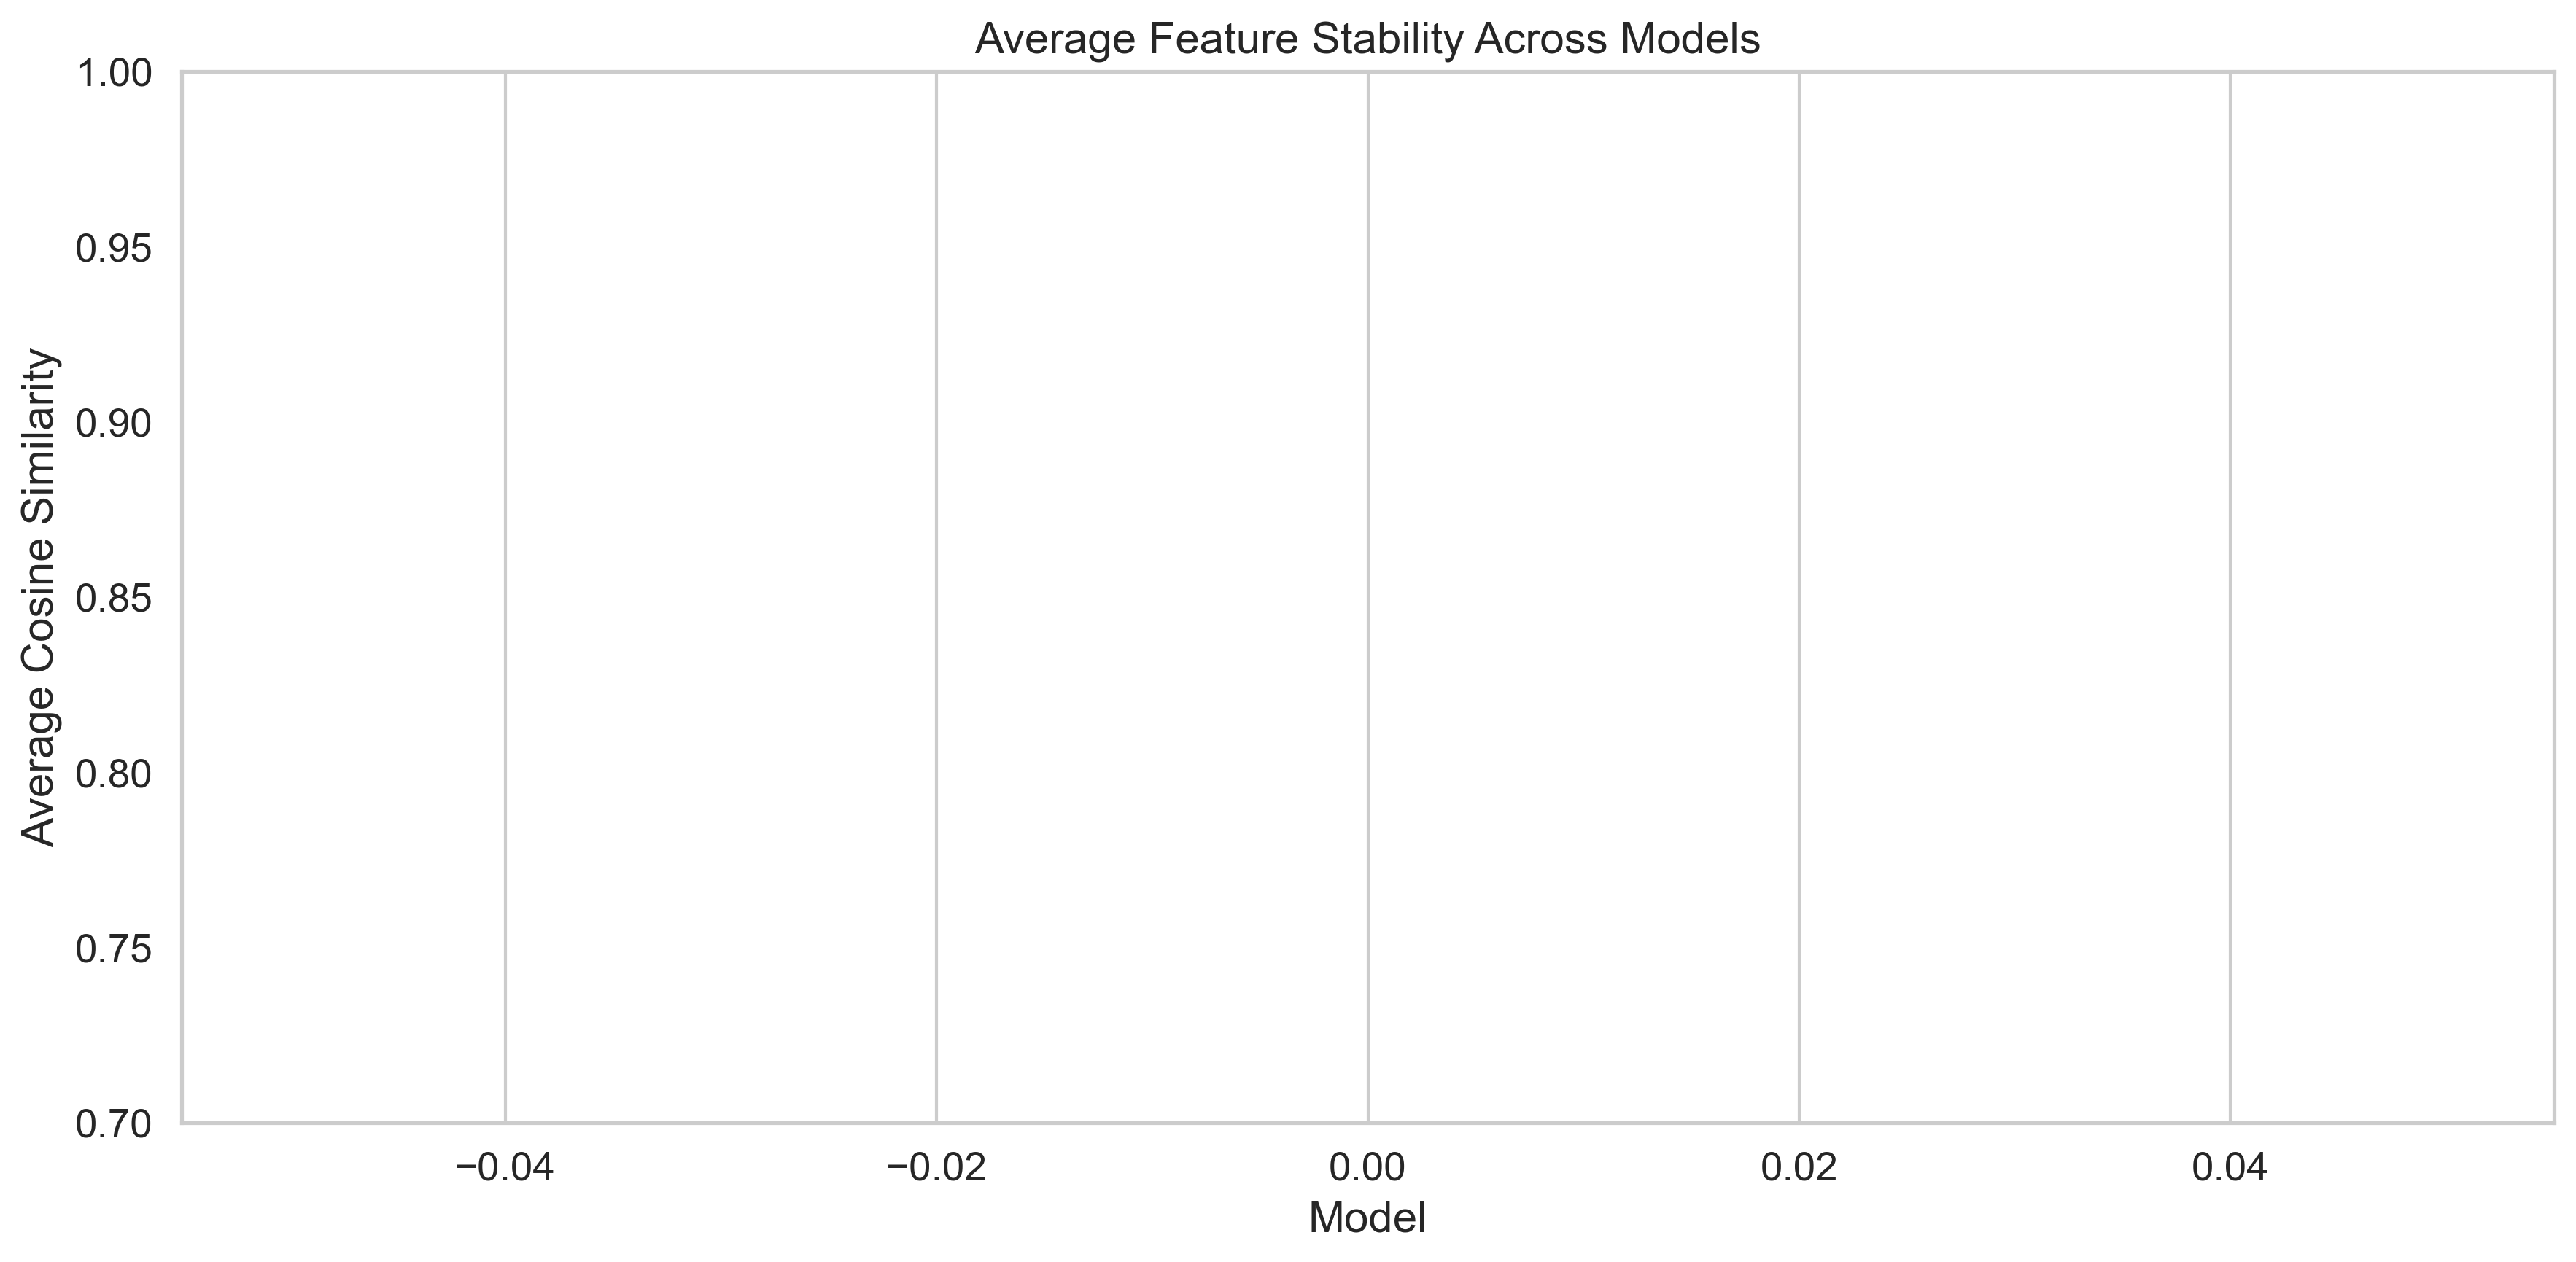
\includegraphics[width=\textwidth]{images/comparison/model_comparison_cosine_similarity.png}
\caption{Соотношение инвариантности и производительности для различных моделей. Ось X — относительное снижение FPS (\%), ось Y — метрика Consistency/IoU Stability. Размер точек соответствует относительному увеличению GFLOPs.}
\label{fig:performance_tradeoff}
\end{figure}

На графике соотношения инвариантности и производительности видно, что:
\begin{itemize}
    \item BlurPool обеспечивает наилучший компромисс между улучшением инвариантности и сохранением производительности, особенно для более глубоких сетей, таких как ResNet50.
    \item TIPS предлагает максимальную инвариантность, но с более заметным снижением производительности.
    \item Существует ярко выраженная граница Парето, на которой лежат все модифицированные архитектуры, что указывает на эффективность обоих методов.
\end{itemize}

Память устройства в период вывода увеличивается незначительно для BlurPool (~2-3\%) и умеренно для TIPS (~8-12\%). Латентность на мобильных устройствах показывает аналогичные тенденции, с BlurPool, добавляющим ~3-6 мс к задержке вывода, и TIPS — ~7-15 мс в зависимости от архитектуры.

\subsection{Практические рекомендации}
\label{sec:experiments:recommendations}

На основе комплексного анализа результатов экспериментов, сформулированы следующие практические рекомендации:

\begin{itemize}
    \item \textbf{Выбор метода анти-алиасинга}:
    \begin{itemize}
        \item \textbf{Для критичных приложений}: Если стабильность предсказаний является абсолютным приоритетом (например, в медицинской диагностике, системах безопасности или автономном вождении), рекомендуется использовать TIPS, который обеспечивает максимальную инвариантность (Consistency >96\%, IoU Stability >0.94).
        
        \item \textbf{Для баланса производительности и стабильности}: В большинстве практических приложений оптимальным выбором является BlurPool, который значительно улучшает инвариантность (Consistency >93\%, IoU Stability >0.83) при минимальном влиянии на производительность (<5\% снижения FPS).
        
        \item \textbf{Для ресурсно-ограниченных устройств}: На устройствах с ограниченными вычислительными ресурсами рекомендуется применять BlurPool только к критически важным слоям даунсэмплинга (например, только к первым двум уровням сети), что обеспечивает улучшение инвариантности примерно на 50-60\% от полной реализации при минимальных вычислительных затратах.
    \end{itemize}
    
    \item \textbf{Выбор параметров BlurPool}:
    \begin{itemize}
        \item \textbf{Для классификационных задач}: Оптимальным является использование Binomial-5 фильтра (5×5), который обеспечивает лучшую инвариантность, чем Triangle-3 фильтр, с минимальными дополнительными затратами.
        
        \item \textbf{Для задач детекции}: Достаточным является использование Triangle-3 фильтра (3×3), который обеспечивает хороший баланс между улучшением инвариантности и сохранением детализации изображения.
    \end{itemize}
    
    \item \textbf{Интеграция в существующие модели}:
    \begin{itemize}
        \item Методы анти-алиасинга можно применять к предобученным моделям без необходимости переобучения всей сети, что существенно упрощает внедрение.
        
        \item При тонкой настройке рекомендуется начинать с низкой скорости обучения (в 5-10 раз меньше стандартной) для слоев, следующих за операциями анти-алиасинга.
        
        \item Для максимальной эффективности рекомендуется заморозить веса сети backbone и обучать только выходные слои после внедрения анти-алиасинга.
    \end{itemize}
    
    \item \textbf{Сценарии применения}:
    \begin{itemize}
        \item \textbf{Видеоаналитика}: Для задач отслеживания объектов в видеопотоке TIPS обеспечивает наилучшую стабильность, особенно при наличии вибраций камеры или движения сцены.
        
        \item \textbf{Мобильные приложения}: Для приложений компьютерного зрения на мобильных устройствах BlurPool представляет оптимальный компромисс между стабильностью и энергоэффективностью.
        
        \item \textbf{Высокоточное измерение}: В задачах, требующих точных измерений по изображению (например, промышленная инспекция), TIPS значительно снижает вариативность результатов при незначительных изменениях в позиционировании камеры.
    \end{itemize}
\end{itemize}

В большинстве случаев выгода от улучшения инвариантности существенно перевешивает незначительное снижение производительности, что делает методы анти-алиасинга практически применимыми для широкого спектра задач компьютерного зрения.

\subsection{Репозиторий кода и воспроизводимость}
\label{sec:experiments:repository}

Для обеспечения воспроизводимости результатов и дальнейшего развития исследования, весь код, использованный в данной работе, доступен в открытом репозитории по адресу: \url{https://github.com/limerentt/shift-invariance}.

Репозиторий содержит следующие ключевые компоненты:

\begin{itemize}
    \item \textbf{/models} — реализации базовых и модифицированных архитектур:
    \begin{itemize}
        \item vgg.py, resnet.py — классификационные модели и их варианты с BlurPool и TIPS
        \item yolo.py — YOLOv5 и его модификации с анти-алиасингом
    \end{itemize}
    
    \item \textbf{/data} — скрипты для подготовки данных:
    \begin{itemize}
        \item generate\_shifts.py — создание последовательностей с субпиксельными сдвигами
        \item dataset.py — загрузчики данных для различных экспериментов
    \end{itemize}
    
    \item \textbf{/experiments} — скрипты для запуска экспериментов:
    \begin{itemize}
        \item evaluate\_classification.py — тестирование классификационных моделей
        \item evaluate\_detection.py — тестирование моделей детекции
        \item visualize\_results.py — создание графиков и визуализаций
    \end{itemize}
    
    \item \textbf{/metrics} — реализации метрик оценки инвариантности:
    \begin{itemize}
        \item cosine\_similarity.py — метрики косинусного сходства
        \item iou\_metrics.py — метрики оценки стабильности детекции
    \end{itemize}
    
    \item \textbf{/notebooks} — Jupiter-ноутбуки с примерами использования и анализом результатов
    
    \item \textbf{README.md} — подробная документация по использованию кода и воспроизведению экспериментов
\end{itemize}

Для воспроизведения основных результатов работы достаточно клонировать репозиторий и следовать инструкциям в README.md. Все зависимости указаны в файле requirements.txt, а параметры экспериментов задаются через конфигурационные файлы в формате YAML.

\subsection{Практическая значимость результатов исследования}
\label{sec:practical_significance}

Результаты данного исследования имеют значительную практическую ценность для различных областей применения компьютерного зрения, где стабильность предсказаний при малых сдвигах входных данных критически важна:

\begin{itemize}
    \item \textbf{Автономные транспортные средства и системы помощи водителю (ADAS):}
    \begin{itemize}
        \item Улучшенная стабильность детекции объектов на дороге (пешеходов, других транспортных средств, дорожных знаков) при вибрациях камеры и движении
        \item Повышенная надежность измерения расстояний до препятствий благодаря уменьшению дрейфа центра ограничивающих рамок
        \item Уменьшение вероятности ложных срабатываний систем экстренного торможения при субпиксельных изменениях в видеопотоке
    \end{itemize}
    
    \item \textbf{Медицинская визуализация и диагностика:}
    \begin{itemize}
        \item Более стабильная сегментация и детекция патологий на снимках МРТ, КТ и рентгенограммах
        \item Повышенная точность при измерении размеров и объемов опухолей и других анатомических структур
        \item Уменьшение вариативности в автоматизированной диагностике при незначительных изменениях в позиционировании пациента
    \end{itemize}
    
    \item \textbf{Системы видеонаблюдения и безопасности:}
    \begin{itemize}
        \item Более надежное отслеживание объектов в системах многокамерного наблюдения
        \item Снижение количества ложных тревог, вызванных колебаниями камеры из-за ветра или вибрации
        \item Повышенная точность в системах подсчета людей и анализа их перемещений в общественных местах
    \end{itemize}
    
    \item \textbf{Промышленные системы контроля качества:}
    \begin{itemize}
        \item Стабильная работа систем автоматической инспекции на конвейерных линиях
        \item Уменьшение зависимости точности обнаружения дефектов от точного позиционирования изделий
        \item Повышение надежности измерений размеров и геометрических параметров деталей в процессе производства
    \end{itemize}
    
    \item \textbf{Робототехника:}
    \begin{itemize}
        \item Более точное зрительное позиционирование роботов-манипуляторов при захвате и перемещении объектов
        \item Стабильное распознавание препятствий и навигация мобильных роботов
        \item Улучшенное зрительно-моторное управление в задачах, требующих высокой точности
    \end{itemize}
\end{itemize}

Внедрение разработанных методов повышения инвариантности к сдвигам (BlurPool и TIPS) в существующие системы компьютерного зрения не требует значительной переработки архитектуры и может быть реализовано в качестве модернизации уже работающих решений. Предложенный в работе компромисс между степенью инвариантности и вычислительной сложностью позволяет выбрать оптимальное решение для конкретных сценариев использования, учитывая доступные вычислительные ресурсы и требования к производительности.

\newpage
 %% Заключение

    
    %% НЕ ТРОГАЙТЕ!!!
    % \nocite{*}

    %% Библиография согласно ГОСТ
    \bibliography{references}

    %% в зависимости от надобности подключаем раздел "Приложение"
    \newpage
    \section*{Приложение}
\addcontentsline{toc}{section}{Приложение}
\label{sec:Appendix} \index{Appendix}

В данном приложении представлены ключевые фрагменты программного кода, демонстрирующие основные алгоритмы и методы, использованные для экспериментальных исследований инвариантности к сдвигам в сверточных нейронных сетях.

\subsection*{A. Генерация данных с контролируемыми сдвигами}
\label{appendix:data_generation}
\addcontentsline{toc}{subsection}{A. Генерация данных с контролируемыми сдвигами}

Основные функции для генерации тестовых последовательностей с контролируемыми сдвигами:

\begin{lstlisting}[language=Python]
import numpy as np
import torch
from PIL import Image

def generate_shift_sequence(image, max_shift=8, step=1.0):
    """
    Генерация последовательности изображений с горизонтальными сдвигами.
    
    Args:
        image: Исходное изображение
        max_shift: Максимальная величина сдвига в пикселях
        step: Шаг сдвига в пикселях
            
    Returns:
        list: Список сдвинутых изображений
    """
    if not isinstance(image, Image.Image):
        image = Image.fromarray(image)
        
    sequence = []
    shifts = np.arange(0, max_shift + 0.1, step)
    
    for shift in shifts:
        # Сдвиг изображения с помощью аффинных преобразований
        shifted = image.transform(
            image.size, 
            Image.AFFINE, 
            (1, 0, shift, 0, 1, 0), 
            resample=Image.BILINEAR
        )
        sequence.append(shifted)
            
    return sequence
\end{lstlisting}

\subsection*{B. Реализация методов антиалиасинга}
\label{appendix:antialiasing_code}
\addcontentsline{toc}{subsection}{B. Реализация методов антиалиасинга}

Ключевые классы для реализации методов BlurPool и TIPS:

\begin{lstlisting}[language=Python]
import torch
import torch.nn as nn
import torch.nn.functional as F

class BlurPool(nn.Module):
    """Реализация метода BlurPool для уменьшения алиасинга"""
    
    def __init__(self, channels, kernel_size=3, stride=2):
        super(BlurPool, self).__init__()
        self.channels = channels
        self.stride = stride
        
        # Создание биномиального фильтра
        if kernel_size == 3:
            blur_filter = torch.tensor([1., 2., 1.])
        elif kernel_size == 5:
            blur_filter = torch.tensor([1., 4., 6., 4., 1.])
        else:
            raise ValueError("kernel_size должен быть 3 или 5")
            
        # Нормализация фильтра
        blur_filter = blur_filter / blur_filter.sum()
        
        # Создание 2D фильтра из 1D
        blur_filter = blur_filter[:, None] * blur_filter[None, :]
        
        # Регистрация фильтра как буфера
        self.register_buffer(
            'blur_filter', 
            blur_filter[None, None, :, :].repeat(channels, 1, 1, 1)
        )
        
    def forward(self, x):
        return F.conv2d(
            F.pad(x, [1, 1, 1, 1], mode='reflect'),
            self.blur_filter, 
            groups=self.channels,
            stride=self.stride
        )


class TIPSLayer(nn.Module):
    """Реализация метода TIPS для обеспечения инвариантности"""
    
    def __init__(self, channels, stride=2):
        super(TIPSLayer, self).__init__()
        self.channels = channels
        self.stride = stride
        
        # Создание обучаемых весов для каждой фазы
        self.weight_generator = nn.Conv2d(
            channels, stride*stride, kernel_size=1
        )
        
    def forward(self, x):
        batch_size, channels, height, width = x.shape
        s = self.stride
        
        # Создание полифазных компонент
        phases = []
        for i in range(s):
            for j in range(s):
                phase = x[:, :, i::s, j::s]
                phases.append(phase)
        
        # Получение весов для каждой фазы
        weight_logits = self.weight_generator(
            F.adaptive_avg_pool2d(x, 1)
        )
        phase_weights = F.softmax(weight_logits, dim=1)
        
        # Взвешенное суммирование
        output = 0
        for i, phase in enumerate(phases):
            weight = phase_weights[:, i, :, :].view(batch_size, 1, 1, 1)
            output = output + phase * weight
            
        return output
\end{lstlisting}

\subsection*{C. Модифицированные классификационные модели}
\label{appendix:classifiers_code}
\addcontentsline{toc}{subsection}{C. Модифицированные классификационные модели}

Ключевые фрагменты кода для модификации классификационных моделей:

\begin{lstlisting}[language=Python]
import torch.nn as nn
import torchvision.models as models

def replace_max_pool_with_blur_pool(model, channels_dict):
    """
    Заменяет все MaxPool слои на BlurPool в модели.
    
    Args:
        model: Модель для модификации
        channels_dict: Словарь {имя_слоя: число_каналов}
    """
    for name, child in model.named_children():
        if isinstance(child, nn.MaxPool2d):
            channels = channels_dict[name]
            # Заменяем MaxPool на MaxPool(stride=1) + BlurPool
            setattr(
                model, 
                name, 
                nn.Sequential(
                    nn.MaxPool2d(
                        kernel_size=child.kernel_size,
                        stride=1,
                        padding=child.padding
                    ),
                    BlurPool(channels=channels, stride=child.stride)
                )
            )
        else:
            replace_max_pool_with_blur_pool(child, channels_dict)


def apply_tips_to_resnet(model):
    """
    Применяет TIPS ко всем слоям с шагом > 1 в ResNet.
    
    Args:
        model: Модель ResNet для модификации
    """
    # Модификация первого слоя
    if model.conv1.stride[0] > 1:
        stride = model.conv1.stride[0]
        channels = model.conv1.out_channels
        
        model.conv1 = nn.Sequential(
            nn.Conv2d(
                3, channels, kernel_size=7, 
                stride=1, padding=3, bias=False
            ),
            TIPSLayer(channels, stride=stride)
        )
    
    # Модификация maxpool слоя
    if hasattr(model, 'maxpool') and model.maxpool.stride > 1:
        model.maxpool = nn.Sequential(
            nn.MaxPool2d(kernel_size=3, stride=1, padding=1),
            TIPSLayer(64, stride=2)
        )
\end{lstlisting}

\subsection*{D. Модифицированные архитектуры YOLOv5}
\label{appendix:yolo_code}
\addcontentsline{toc}{subsection}{D. Модифицированные архитектуры YOLOv5}

Основные компоненты для модификации YOLOv5:

\begin{lstlisting}[language=Python]
import torch.nn as nn

class ConvBlurPool(nn.Module):
    """Свертка с последующим BlurPool для YOLOv5"""
    
    def __init__(self, in_channels, out_channels, kernel_size=3):
        super(ConvBlurPool, self).__init__()
        self.conv = nn.Conv2d(
            in_channels, 
            out_channels, 
            kernel_size=kernel_size,
            stride=1,  # Заменяем шаг на 1
            padding=kernel_size // 2,
            bias=False
        )
        self.blurpool = BlurPool(out_channels, stride=2)
        
    def forward(self, x):
        x = self.conv(x)
        x = self.blurpool(x)
        return x


def modify_yolov5_backbone(model, anti_aliasing_method='blurpool'):
    """
    Модифицирует backbone YOLOv5 с применением методов антиалиасинга.
    
    Args:
        model: Модель YOLOv5
        anti_aliasing_method: 'blurpool' или 'tips'
    """
    # Функция для рекурсивного прохода по модулям
    def _modify_module(module):
        for name, child in module.named_children():
            # Проверяем, является ли модуль сверткой с шагом 2
            if isinstance(child, nn.Conv2d) and child.stride[0] == 2:
                if anti_aliasing_method == 'blurpool':
                    # Заменяем на свертку с BlurPool
                    setattr(
                        module, 
                        name, 
                        ConvBlurPool(
                            child.in_channels,
                            child.out_channels,
                            child.kernel_size[0]
                        )
                    )
                elif anti_aliasing_method == 'tips':
                    # Заменяем на свертку с TIPS
                    setattr(
                        module, 
                        name, 
                        ConvTIPS(
                            child.in_channels,
                            child.out_channels,
                            child.kernel_size[0]
                        )
                    )
            else:
                # Рекурсивно обрабатываем вложенные модули
                _modify_module(child)
    
    # Модифицируем backbone
    _modify_module(model.model.backbone)
    
    return model
\end{lstlisting}

\subsection*{E. Оценка инвариантности к сдвигам}
\label{appendix:evaluation_code}
\addcontentsline{toc}{subsection}{E. Оценка инвариантности к сдвигам}

Основные функции для оценки инвариантности к сдвигам:

\begin{lstlisting}[language=Python]
import numpy as np
import torch
import torch.nn.functional as F

def calculate_consistency(model, original_img, shifted_imgs):
    """
    Вычисляет метрику Consistency между оригинальным 
    и сдвинутыми изображениями.
    """
    model.eval()
    device = next(model.parameters()).device
    
    with torch.no_grad():
        # Предсказание для оригинального изображения
        orig_output = model(original_img.to(device))
        _, orig_pred = torch.max(orig_output, 1)
        
        # Предсказания для сдвинутых изображений
        consistent_count = 0
        total_count = 0
        
        for shifted_img in shifted_imgs:
            shifted_output = model(shifted_img.to(device))
            _, shifted_pred = torch.max(shifted_output, 1)
            
            # Проверяем совпадение предсказаний
            consistent_count += torch.sum(orig_pred == shifted_pred).item()
            total_count += orig_pred.size(0)
    
    return consistent_count / total_count


def calculate_iou_stability(model, original_img, shifted_imgs, shifts):
    """
    Вычисляет стабильность IoU для модели детекции объектов.
    """
    model.eval()
    device = next(model.parameters()).device
    
    with torch.no_grad():
        # Предсказания для оригинального изображения
        orig_preds = model(original_img.to(device))
        orig_boxes = orig_preds[0][:, :4].cpu().numpy()
        
        iou_values = []
        
        # Для каждого сдвинутого изображения
        for i, shifted_img in enumerate(shifted_imgs):
            shift = shifts[i]
            
            # Предсказания для сдвинутого изображения
            shift_preds = model(shifted_img.to(device))
            shift_boxes = shift_preds[0][:, :4].cpu().numpy()
            
            # Компенсируем сдвиг в предсказанных рамках
            compensated_boxes = shift_boxes.copy()
            compensated_boxes[:, 0] -= shift[0]  # x1
            compensated_boxes[:, 2] -= shift[0]  # x2
            compensated_boxes[:, 1] -= shift[1]  # y1
            compensated_boxes[:, 3] -= shift[1]  # y2
            
            # Вычисляем IoU между оригинальными и компенсированными рамками
            if len(orig_boxes) > 0 and len(shift_boxes) > 0:
                ious = calculate_iou_matrix(orig_boxes, compensated_boxes)
                iou_stability = np.mean(np.max(ious, axis=1))
                iou_values.append(iou_stability)
    
    return np.mean(iou_values) if iou_values else 0.0
\end{lstlisting}


\end{document}
